% ============================================================
%  Literature Survey: Architectural Failures in Spatio-Temporal
%  Graph and Federated Learning Models for Financial Fraud Detection
% ============================================================
\documentclass[12pt, a4paper]{article}

% ── Packages ─────────────────────────────────────────────────
\usepackage[T1]{fontenc}
\usepackage[utf8]{inputenc}
\usepackage{lmodern}
\usepackage{microtype}
\usepackage{geometry}
\geometry{
  a4paper,
  top=2.5cm, bottom=2.5cm,
  left=2.5cm, right=2.5cm
}
\usepackage{setspace}
\setstretch{1.25}

\usepackage{titlesec}
\usepackage[table]{xcolor}
\usepackage{booktabs}
\usepackage{longtable}
\usepackage{array}
\usepackage{tabularx}
\usepackage{ragged2e}
\usepackage{parskip}
\usepackage{enumitem}
\usepackage{hyperref}
\usepackage{amsmath}
\usepackage{placeins}
\usepackage{fancyhdr}
\usepackage{graphicx}
\usepackage[backend=biber, style=numeric, sorting=nyt, maxbibnames=99, defernumbers=false]{biblatex}
\addbibresource{literature_survey.bib}

% ── Force numbered labels in the printed bibliography ─────
\DeclareFieldFormat{labelnumberwidth}{\mkbibbrackets{#1}}
\setlength{\biblabelsep}{8pt}
\setlength{\bibitemsep}{6pt}

% ── Colours ──────────────────────────────────────────────────
\definecolor{navyblue}{RGB}{31, 56, 100}
\definecolor{lightblue}{RGB}{214, 228, 240}
\definecolor{rowgray}{RGB}{245, 248, 252}
\definecolor{accent}{RGB}{41, 128, 185}

% ── Section / subsection formatting ──────────────────────────
\titleformat{\section}
  {\large\bfseries\color{navyblue}}
  {\thesection.}{0.6em}{}[\vspace{-4pt}\textcolor{navyblue}{\rule{\linewidth}{1pt}}]

\titleformat{\subsection}
  {\normalsize\bfseries\color{navyblue}}
  {\thesubsection}{0.5em}{}

\titlespacing{\section}{0pt}{18pt}{8pt}
\titlespacing{\subsection}{0pt}{12pt}{4pt}

% ── Header / Footer ──────────────────────────────────────────
\pagestyle{fancy}
\fancyhf{}
\fancyhead[L]{\small\color{navyblue}\textbf{Methodology}}
\fancyhead[R]{\small\color{navyblue}GNN \& Federated Learning, 2022--2025}
\fancyfoot[C]{\small\thepage}
\renewcommand{\headrulewidth}{0.4pt}
\renewcommand{\headrule}{\hbox to\headwidth{\color{navyblue}\leaders\hrule height \headrulewidth\hfill}}

% ── Survey entry environment ─────────────────────────────────
\newenvironment{surveyentry}[1]{%
  \vspace{6pt}
  \noindent\textbf{\color{navyblue}#1}\par
  \vspace{2pt}
  \noindent\hspace{1em}%
  \begin{minipage}[t]{0.97\linewidth}
}{%
  \end{minipage}
  \vspace{10pt}
}

% ── Table column types ────────────────────────────────────────
\newcolumntype{L}[1]{>{\RaggedRight\arraybackslash}p{#1}}

% ── Hyperlink setup ───────────────────────────────────────────
\hypersetup{
  colorlinks = true,
  linkcolor  = navyblue,
  citecolor  = accent,
  urlcolor   = accent
}

% ═════════════════════════════════════════════════════════════
\begin{document}

% ── Title block ──────────────────────────────────────────────
\begin{center}
  {\LARGE\bfseries\color{navyblue}
    Methodology}\\[6pt]
  {\large\bfseries\color{navyblue}
    Architectural Failures in Spatio-Temporal Graph and\\
    Federated Learning Models for Financial Fraud Detection}\\[8pt]
  {\normalsize\itshape\color{gray}
    A critical survey of GNN, STGNN, and Federated Learning architectures, 2022--2025}\\[10pt]

  % ── Authors block ────────────────────────────────────────
  \renewcommand{\arraystretch}{1.3}
  \begin{tabular}{@{}p{3.4cm}p{3.2cm}p{3.4cm}p{3.4cm}@{}}
    \centering\textbf{Aditanshu Sahu} &
    \centering\textbf{Adina Haseeb} &
    \centering\textbf{Aditya Singh} &
    \centering\textbf{Aditya Verma}\tabularnewline[1pt]
    \centering{\footnotesize 230953444} &
    \centering{\footnotesize 230953096} &
    \centering{\footnotesize 230953458} &
    \centering{\footnotesize 230953432}\tabularnewline[1pt]
    \centering{\tiny\ttfamily\color{accent}aditanshu.mitmpl2023\newline @learner.manipal.edu} &
    \centering{\tiny\ttfamily\color{accent}ada.mitmpl2023\newline @learner.manipal.edu} &
    \centering{\tiny\ttfamily\color{accent}aditya29.mitmpl2023\newline @learner.manipal.edu} &
    \centering{\tiny\ttfamily\color{accent}aditya28.mitmpl2023\newline @learner.manipal.edu}\tabularnewline[1pt]
    \centering{\footnotesize\href{https://wa.me/919321611281}{+91\,9321611281}} &
    \centering{---} &
    \centering{---} &
    \centering{---}\tabularnewline
  \end{tabular}\\[10pt]
 
  {\small\color{gray}\today}
\end{center}
 
\vspace{4pt}
{\color{navyblue}\rule{\linewidth}{1.5pt}}
\vspace{14pt}

% ═══════════════════════════════════════════════════════════
\section{Introduction}
% ═══════════════════════════════════════════════════════════

This literature survey systematically reviews the major research contributions related to the critical analysis of architectural failures in spatio-temporal graph and federated learning models for financial fraud detection. The global shift toward real-time digital payment systems---including UPI, FedNow, and SEPA Instant---has reduced the fraud detection window to milliseconds, rendering legacy rule-based and tabular machine learning frameworks insufficient. Researchers have consequently pivoted toward Graph Neural Networks (GNNs), Spatio-Temporal Graph Neural Networks (STGNNs), and Federated Learning (FL) as the next generation of fraud detection architectures.

However, by 2024 and 2025, a series of critical vulnerabilities in these architectures have been identified, including sensitivity to data drift, gradient-based privacy leakage, real-time computational bottlenecks, and regulatory non-compliance with the EU AI Act and DORA. The following survey entries, organised thematically, cover every major topic addressed in the source material---from foundational relational modelling and real-time pipeline challenges to privacy paradoxes in federated learning and the regulatory landscape.

% ═══════════════════════════════════════════════════════════
\section{Foundational GNN Architectures for Spatial-Temporal Fraud Detection}
% ═══════════════════════════════════════════════════════════

\subsection*{Entry 1: Cheng, Wang, Zhang, and Zhang (2022)}

\begin{surveyentry}{Citation: \cite{cheng2022stagn}}
\cite{cheng2022stagn} addressed the challenge of automatically capturing the most relevant fraudulent behavioural patterns in online credit card fraud detection without relying on domain-specific manual feature engineering. They constructed a transaction graph using real-world credit card records, encoding location- and time-stamped relationships as spatial and temporal edges between cardholders, merchants, and devices. \cite{cheng2022stagn} trained a Spatial-Temporal Attention-based Graph Network (STAGN) that first applied a GNN to learn transaction graph features and then applied spatial-temporal attention on top of the learned tensor representations, which were fed into a 3D convolution network; attention weights were jointly optimised end-to-end with the detection network. The authors reported that STAGN outperformed all state-of-the-art baselines in AUC and precision-recall curves, demonstrating superiority in detecting suspicious transactions and uncovering spatial and temporal fraud hotspots. The attention mechanism is limited by high computational cost, which restricts scalable deployment in real-time streaming payment systems.
\end{surveyentry}

\subsection*{Entry 2: Gummadi (2025)}

\begin{surveyentry}{Citation: \cite{gummadi2025temporal}}
\cite{gummadi2025temporal} addressed the problem of capturing temporal dependencies and relational patterns in real-time, multi-national cross-border payment transactions that are increasingly vulnerable to coordinated fraud attacks evolving rapidly over time. He constructed streaming, multi-national payment graphs with dynamic node embeddings, applying time-aware message passing across transaction nodes to capture both short-term anomalies and long-range dependencies within live payment data. \cite{gummadi2025temporal} applied Temporal Graph Neural Networks (TGNNs) with a streaming graph architecture, encoding temporal state transitions directly into node embeddings that were updated continuously as new transactions arrived; the framework was evaluated on simulated cross-border payment streams. He reported that the TGNN framework effectively detected evolving fraudulent behaviour in streaming multi-national datasets, with the temporal node embeddings capturing both localised transaction bursts and long-horizon behavioural deviations. The model is limited by scalability constraints when transaction volumes reach thousands of events per second in high-velocity international payment corridors.
\end{surveyentry}

\subsection*{Entry 3: Harper and Lee (2025)}

\begin{surveyentry}{Citation: \cite{harper2025blockchain}}
\cite{harper2025blockchain} addressed the challenge that traditional fraud detection techniques---rule-based systems and supervised machine learning models---struggle with the high-volume, high-velocity, and dynamically evolving nature of blockchain transactions, particularly for detecting money laundering, Ponzi schemes, and illicit fund transfers. They modelled blockchain transactions as a spatial-temporal graph, representing wallets as nodes and fund movements as temporal edges, and extracted both spatial dependencies among wallets and temporal patterns of fund movements from a large-scale blockchain network. \cite{harper2025blockchain} employed a Spatial-Temporal Graph Neural Network (STGNN) that used GCN or GAT layers for spatial feature extraction and a Gated Recurrent Unit (GRU) for temporal feature modelling; they evaluated the framework on large-scale blockchain datasets to measure anomaly detection effectiveness. They reported enhanced security and resilience in blockchain networks against fraudulent and malicious operations, demonstrating that the STGNN's combination of spatial relationship learning and temporal pattern modelling substantially outperformed non-relational baselines. The computational overhead of training and performing inference on deep STGNNs is limiting for real-time blockchain validation in environments with strict sub-200\,ms latency requirements.
\end{surveyentry}

% ═══════════════════════════════════════════════════════════
\section{GNN Robustness Failures Under Data Drift}
% ═══════════════════════════════════════════════════════════

\subsection*{Entry 4: IEEE Access Data Drift Study (2025)}

\begin{surveyentry}{Citation: \cite{ieeeaccess2025drift}}
\cite{ieeeaccess2025drift} addressed the underexplored problem of GNN robustness to natural, temporal data drift in the financial fraud detection domain, where adversarial behaviours and consumer patterns change continuously and existing models are typically trained on historical static graphs. They used the large-scale, highly imbalanced IEEE-CIS Fraud Detection benchmark dataset, constructing homogeneous transaction graphs and applying a strict temporal data-splitting methodology to simulate a realistic deployment scenario where models must generalise to future, unseen data distributions. The researchers evaluated three foundational GNN architectures---Graph Convolutional Networks (GCNs), Graph Attention Networks (GATs), and Graph Sample and Aggregate (GraphSAGE)---over 50 sequential, non-overlapping monitoring windows, using AUC-PR and F2-Score as primary metrics due to their sensitivity in heavily imbalanced class distributions. They reported that all three evaluated GNNs suffered from significant performance degradation over time, with GCN and GAT showing pronounced declines, while GraphSAGE demonstrated substantially greater robustness because its inductive sampling approach allowed it to generalise better to new nodes and evolving edge structures. The study is limited by the absence of an adaptive retraining mechanism; it diagnoses the degradation phenomenon but does not propose a mitigation strategy to restore model performance during concept drift.
\end{surveyentry}

\subsection*{Entry 5: Kazim (2025)}

\begin{surveyentry}{Citation: \cite{kazim2025drift}}
\cite{kazim2025drift} addressed the critical and often invisible risk of AI model drift in financial institutions, arguing that macroeconomic shocks---such as sudden tariff changes and stock market volatility in mid-2025---expose systemic fragility in AI models trained on historically stable data. He analysed the impact of US tariff announcements from April 2025 on bank AI systems, drawing on industry data, regulatory events, and case studies of institutions penalised by the European Central Bank for deploying outdated anti-money-laundering models. Kazim used a conceptual and policy analysis framework, synthesising evidence from the EU AI Act, the US Federal Reserve SR 11-7 model risk guidance, and empirical reports of bank stock declines and credit risk model failures caused by macroeconomic shifts triggering concept drift in previously reliable AI systems. He reported that models calibrated on 2024 stable economic data were found to fail significantly under 2025 market conditions, that the ECB fined three banks for using outdated models, and that institutions without transparent retraining protocols face both regulatory penalties and consequential financial exposure exceeding \$500 million annually for top banks. The adoption of rigorous drift monitoring, lifecycle management, and retraining protocols across financial institutions is limited by regulatory uncertainty, legacy infrastructure constraints, and the significant engineering effort required to implement continuous model performance auditing.
\end{surveyentry}

% ═══════════════════════════════════════════════════════════
\section{Spatio-Temporal Propagation Conflation and Real-Time Pipeline Failures}
% ═══════════════════════════════════════════════════════════

\subsection*{Entry 6: HST-GAT Study---MDPI Processes (2025)}

\begin{surveyentry}{Citation: \cite{hstgat2025mdpi}}
\cite{hstgat2025mdpi} addressed the theoretical shortfall in hybrid STGNN architectures where spatial anomaly propagation---one compromised entity infecting its graph neighbourhood---and temporal state transitions---the network evolving over time---are conflated into a single aggregated representation by naively stacking Recurrent Neural Network (RNN) layers on GNN layers. They constructed a two-stage hierarchical model architecture evaluated on anomaly detection benchmarks, where each stage was dedicated to explicitly modelling either spatial spread or temporal evolution separately, rather than merging them in a shared representation space. The authors proposed the Hierarchical Spatio-Temporal Graph Attention Network (HST-GAT), which employs a dedicated spatial graph attention sub-network followed by a separate temporal attention sub-network, allowing each component to specialise in one propagation process and produce non-conflated, interpretable risk representations. They reported that HST-GAT produced cleaner, more interpretable risk signals than na\"{i}ve GNN-RNN stacking approaches, demonstrating improved detection rates for spatially spreading and temporally evolving anomalies across benchmark datasets. The model is limited by high GPU and memory requirements arising from running two sequential attention sub-networks, which restricts deployment in latency-constrained real-time financial transaction scoring pipelines.
\end{surveyentry}

% ═══════════════════════════════════════════════════════════
\section{Federated Learning: Non-IID Divergence and Privacy Paradoxes}
% ═══════════════════════════════════════════════════════════

\subsection*{Entry 7: Sun (2025)}

\begin{surveyentry}{Citation: \cite{sun2025flfraud}}
\cite{sun2025flfraud} addressed the fundamental challenge of applying Federated Learning (FL) for detecting fraud across different financial bodies that have heterogeneous, Non-Independent and Identically Distributed (non-IID) data, where each participating institution has a unique customer base leading to label skew and feature skew that destabilises collaborative training. He used simulated multi-institution financial data distributed across federated clients with varying fraud prevalence rates, evaluating three machine learning models---Artificial Neural Networks (ANN), Random Forest (RF), and Convolutional Neural Networks (CNN)---under the FL framework to assess their communication efficiency, convergence behaviour, and resilience to non-IID data conditions. \cite{sun2025flfraud} compared the federated training dynamics of ANN, RF, and CNN models by measuring their ability to converge to a stable global model under non-IID data partitions, evaluating the trade-off between model complexity, overfitting risk, and communication overhead across federated rounds. He reported that while ANN and CNN demonstrated strong capacity for identifying complex fraud patterns, they suffered from significant communication efficiency challenges and overfitting risks in the federated non-IID context; by contrast, RF offered greater robustness to non-IID data distributions and was less prone to overfitting, although its gradient communication overhead remained a barrier to large-scale deployment. The communication overhead of exchanging high-dimensional model updates across federated institutions is limiting, particularly for Random Forest ensembles in large multi-bank deployments where bandwidth and synchronisation constraints become critical.
\end{surveyentry}

\subsection*{Entry 8: Du, Hu, Wang, Sun, Gong, Ren, and Chen (2025)}

\begin{surveyentry}{Citation: \cite{du2025hcgla}}
\cite{du2025hcgla} addressed the critical and understudied gap between theoretical demonstrations of Gradient Inversion Attack (GIA) effectiveness under ideal laboratory conditions and their actual threat level against practical, production-grade federated learning systems deployed by financial institutions. They systematically surveyed the evolution of GIAs from the original Deep Leakage from Gradients (DLG) framework through to the most recent Highly Compressed Gradient Leakage Attack (HCGLA), constructing an attack timeline and systematisation that identified three fundamental aspects influencing GIA effectiveness: training setup, network architecture, and defence mechanisms. \cite{du2025hcgla} evaluated GIAs across multiple FL configurations, quantifying their ability to reconstruct private training data---including sensitive financial features---from model gradients shared during standard federated aggregation rounds; the HCGLA demonstrated the capability to reconstruct training data from gradients compressed by 99.9\%, representing a 700-fold improvement over 2023 attack performance. The optimisation objective minimised the distance between dummy gradients $\nabla W^{*}$ and the true shared gradients $\nabla W$:
\[
  \arg\min_{x^{*},\, y^{*}} \;\bigl\| \nabla W^{*}(\theta,\, x^{*},\, y^{*}) - \nabla W \bigr\|^{2}
\]
where $\theta$ represents the model parameters and $(x^{*}, y^{*})$ the reconstructed training data \cite{du2025hcgla}. They reported that the HCGLA could extract semantically meaningful private transaction data from shared gradient vectors in deep fraud detection models. The existing defences against the most potent GIA variants in deep federated neural network architectures are limited in both robustness and practical deployability, leaving a significant security gap for financial institutions using standard FedAvg-based collaborative training.
\end{surveyentry}

% ═══════════════════════════════════════════════════════════
\section{Privacy-Preserving Mitigations and Resilient Architecture Designs}
% ═══════════════════════════════════════════════════════════

\subsection*{Entry 9: Guo, Chen, Li, and Geng (2025)}

\begin{surveyentry}{Citation: \cite{guo2025sdpfgs}}
\cite{guo2025sdpfgs} addressed the dual threat in federated learning systems where an untrustworthy central server may both infer clients' private identity information and local training data from received model parameters, and may also falsify aggregation results, thereby compromising both the privacy of individual institutions and the integrity of the globally trained fraud detection model. They designed a federated learning system with a trusted shuffler component that coordinates the parameter fragmentation and group shuffling protocol, evaluating the scheme against a passive honest-but-curious server threat model on benchmark classification tasks to measure privacy preservation and model accuracy retention. \cite{guo2025sdpfgs} proposed the Security Defence scheme based on Parameter Fragmentation and Group Shuffling (SDPFGS), which divides each client's model parameters into multiple fragments, applies differential privacy perturbation to each fragment independently, and then shuffles these fragments across different client groups before submission to the server, so that no attacker can reconstruct a full model update or link fragments to specific clients. They reported that SDPFGS successfully resisted model parameter inversion attacks by untrustworthy servers without degrading the quality of shared model parameters, providing provable anonymity through the shuffling step and maintaining model convergence quality comparable to unprotected federated baselines. The additional shuffling coordination overhead and per-fragment perturbation latency are limiting for very large federated networks with hundreds of participating financial institutions and tight training synchronisation schedules.
\end{surveyentry}

\subsection*{Entry 10: FED-SPFD Study---MDPI Risks (2025)}

\begin{surveyentry}{Citation: \cite{fedspfd2025mdpi}}
\cite{fedspfd2025mdpi} addressed the compounding failures of non-IID statistical heterogeneity and gradient inversion privacy risks in federated credit card fraud detection, where current federated approaches fail to account for the divergence in data distributions across participating banks while simultaneously remaining vulnerable to gradient-based reconstruction attacks. They used multi-party heterogeneous credit card transaction datasets spanning multiple simulated banking institutions with distinct customer bases and fraud prevalence rates, segmenting features into shared fraud-relevant attributes and institution-specific private attributes to reflect the realistic data landscape of a cross-institutional FL deployment. The authors proposed the FED-SPFD model, which employs a share-private feature segmentation approach using a private autoencoder to learn institution-specific feature representations, while aligning on shared features through Local Sufficient Statistics (mean and covariance) rather than raw gradients, thereby collaboratively training a unified fraud detection model without exposing private transaction-level data to the central aggregator. They reported that FED-SPFD improved fraud detection accuracy under heterogeneous data conditions compared to standard FedAvg baselines, and demonstrated greater resilience against gradient inversion attacks by substituting raw gradients with summary statistics that carry insufficient detail for training data reconstruction. The Local Sufficient Statistics alignment mechanism is limited when feature distributions diverge sharply across very heterogeneous institutions where even aggregate statistics reveal sensitive distributional information about the institution's client portfolio.
\end{surveyentry}

% ═══════════════════════════════════════════════════════════
\section{Regulatory Compliance Failures: EU AI Act and DORA}
% ═══════════════════════════════════════════════════════════

A critical and increasingly prominent dimension of architectural failure in financial AI systems in 2024--2025 is non-compliance with emerging regulatory frameworks \cite{euaiact2024,dora2025}. The EU AI Act explicitly classifies AI systems used for credit scoring and fraud detection as \textit{high-risk} when they significantly impact financial transactions or involve profiling, mandating Technical Documentation for complete traceability and Transparency requirements so that users can understand how decisions are formulated \cite{euaiact2024}.

GNNs and STGNNs face a fundamental architectural failure in this regard: the non-linear aggregation of features across multiple hops makes it nearly impossible for a risk officer to explain why a specific transaction was flagged---an \textit{explainability gap} that is a primary barrier to regulatory deployment \cite{kazim2025drift}. While tools such as SHAP values and counterfactual explanations have been integrated into some GNN frameworks to address this gap, they often struggle with the relational nature of graph-based data, where explaining a decision based on a node's multi-hop neighbourhood is fundamentally more complex than explaining a tabular feature-based decision \cite{ieeeaccess2025drift}.

The Digital Operational Resilience Act (DORA) further classifies AI models as part of Information and Communication Technology (ICT) risk management, requiring financial institutions to maintain clear Exit Strategies and continuous Lifecycle Management for deployed models \cite{dora2025}. An architectural failure occurs when a complex STGNN cannot be easily decommissioned or when its model drift cannot be continuously monitored and mitigated---a requirement that static, monolithically trained models cannot satisfy. The European Central Bank has already begun penalising institutions for using outdated models that failed to account for shifting market dynamics \cite{kazim2025drift}.

% ═══════════════════════════════════════════════════════════
\section{Comparative Summary Table}
% ═══════════════════════════════════════════════════════════

Table~\ref{tab:summary} presents a unified comparative summary of all ten reviewed works, including their classifiers, key contributions, and study limitations stated in the present tense.

\vspace{8pt}
\begin{longtable}{%
  L{2.8cm}  % Author(s)
  L{0.7cm}  % Year
  L{3.2cm}  % Classifier
  L{4.5cm}  % Key Contribution
  L{3.5cm}  % Limitation
}
\caption{Comparative Summary of Reviewed Studies (2022--2025)}
\label{tab:summary}\\

\toprule
\textbf{\color{navyblue}Author(s)} &
\textbf{\color{navyblue}Year} &
\textbf{\color{navyblue}Classifiers / Models} &
\textbf{\color{navyblue}Key Contribution} &
\textbf{\color{navyblue}Study Limitation (present tense)} \\
\midrule
\endfirsthead

\multicolumn{5}{l}{\small\itshape (Table~\ref{tab:summary} continued)}\\
\toprule
\textbf{\color{navyblue}Author(s)} &
\textbf{\color{navyblue}Year} &
\textbf{\color{navyblue}Classifiers / Models} &
\textbf{\color{navyblue}Key Contribution} &
\textbf{\color{navyblue}Study Limitation (present tense)} \\
\midrule
\endhead

\bottomrule
\endfoot

\rowcolor{rowgray}
Cheng, Wang, Zhang \& Zhang &
2022 &
STAGN (GNN + Spatial-Temporal Attention + 3D CNN) &
End-to-end spatial-temporal attention graph network detecting fraud hotspots in credit card transaction graphs without manual feature engineering &
Attention computation is limited by high cost in real-time streaming deployment \\

Harper \& Lee &
2025 &
STGNN (GCN/GAT + GRU) &
Spatial-temporal graph framework for large-scale blockchain anomaly detection targeting money laundering and Ponzi schemes &
Computational overhead of deep STGNN inference is limiting for real-time blockchain validation \\

\rowcolor{rowgray}
Gummadi &
2025 &
Temporal GNN (TGNN) with time-aware message passing &
Time-aware node embeddings for streaming, multi-national cross-border payment fraud detection &
Scalability to ultra-high transaction volumes is limiting \\

IEEE Access study &
2025 &
GCN, GAT, GraphSAGE (comparative) &
First systematic study of GNN robustness to data drift on the IEEE-CIS dataset over 50 sequential monitoring windows; reveals GraphSAGE superiority &
No adaptive retraining mechanism is incorporated; degradation under concept drift is not yet mitigated \\

\rowcolor{rowgray}
Kazim &
2025 &
Conceptual / policy analysis &
Identifies macroeconomic shock-triggered AI model drift as a critical systemic risk to financial institution AI systems under the EU AI Act and SR 11-7 &
Practical drift-monitoring frameworks and retraining protocols are still nascent and are limited by regulatory uncertainty \\

HST-GAT study (MDPI) &
2025 &
Hierarchical Spatio-Temporal Graph Attention Network (HST-GAT) &
Two-stage architecture separating spatial propagation and temporal state transitions to eliminate conflation artefacts in anomaly detection &
High GPU and memory requirements from two sequential attention sub-networks are limiting for real-time deployment \\

\rowcolor{rowgray}
Sun &
2025 &
ANN, Random Forest, CNN (in federated setting) &
Comparative study of ML models in FL context; demonstrates RF superior robustness to non-IID data and reduced overfitting risk in decentralised fraud detection &
Communication overhead of gradient exchange in federated RF is limiting for large-scale multi-bank deployment \\

Du, Hu, Wang, Sun, Gong, Ren \& Chen &
2025 &
Gradient Inversion Attack (HCGLA) framework across multiple FL architectures &
Comprehensive SoK of gradient inversion attacks; introduces HCGLA capable of reconstructing private data from gradients compressed by 99.9\% &
Defence evaluation against the most potent GIA variants in deep FL architectures is limited \\

\rowcolor{rowgray}
Guo, Chen, Li \& Geng &
2025 &
Federated Learning + Differential Privacy + Group Shuffling (SDPFGS) &
Parameter fragmentation + DP perturbation + group shuffling to resist malicious server inference attacks in federated fraud detection &
Additional shuffling latency and coordination cost are limiting for very large federated networks \\

FED-SPFD study (MDPI Risks) &
2025 &
Federated Learning + Share-Private Autoencoder (FED-SPFD) &
Share-private feature segmentation with Local Sufficient Statistics alignment to counter non-IID skew and gradient inversion attacks simultaneously &
Alignment via summary statistics is limited when feature distributions diverge sharply across very heterogeneous institutions \\

\end{longtable}

% ═══════════════════════════════════════════════════════════
\section{Synthesis and Conclusion}
% ═══════════════════════════════════════════════════════════

The studies reviewed in this survey collectively reveal a field at a critical inflection point. GNNs and STGNNs have established clear theoretical and empirical superiority over legacy tabular models in detecting complex, multi-hop fraud rings; however, this superiority comes at the cost of robustness, explainability, and operational stability. \cite{cheng2022stagn} laid the foundational architecture for spatial-temporal fraud modelling, while \cite{gummadi2025temporal} and \cite{harper2025blockchain} extended this to cross-border and blockchain contexts respectively, demonstrating the breadth of STGNN applicability.

The data drift findings---particularly the IEEE Access investigation \cite{ieeeaccess2025drift} and Kazim \cite{kazim2025drift} macroeconomic analysis---establish that concept drift is not an edge case but a persistent and systemic challenge that all deployed GNN models will encounter. In the federated domain, \cite{du2025hcgla}'s SoK and the FED-SPFD study \cite{fedspfd2025mdpi} expose the paradox at the heart of privacy-preserving collaborative learning: the gradients that federated learning exchanges are not truly private, and even highly compressed versions remain exploitable. \cite{guo2025sdpfgs}'s SDPFGS and the FED-SPFD model represent the current frontier of mitigation, but both acknowledge residual limitations under adversarial conditions or extreme feature heterogeneity.

\cite{sun2025flfraud}'s comparative study provides actionable insight for practitioners, confirming that simpler models like Random Forest can outperform deep learning in federated non-IID environments when communication efficiency and overfitting resistance are prioritised. Finally, the regulatory dimension---the EU AI Act's high-risk classification \cite{euaiact2024} and DORA's lifecycle management requirements \cite{dora2025}---adds a layer of non-technical failure risk that is increasingly as consequential as predictive accuracy. The next generation of resilient financial fraud detection must be inductive, decoupled, privacy-tiered, and explainable by design.


% ═══════════════════════════════════════════════════════════

\section{Methodology}
% ═══════════════════════════════════════════════════════════
 
This chapter presents a hybrid methodological framework combining Spatio-Temporal Graph Neural Networks (STGNNs), Federated Learning (FL), and drift-aware monitoring mechanisms to deliver a secure and privacy-preserving solution for detecting financial frauds of today. It is a direct intervention to the identified architectural failures through literature survey in the preceding chapters. It merges inductive graph learning, temporal sequence modelling, and privacy-preserving aggregation into a single, regulation-compliant pipeline.
 
% ─────────────────────────────────────────────────────────────
\subsection{A.\quad Overall System Architecture}
% ─────────────────────────────────────────────────────────────
 
The proposed architecture has been planned as a multilayered pipeline following an Input $\rightarrow$ Processing $\rightarrow$ Output flow. It is optimised for distributed environments where data are localised at each participating financial institution \cite{flfraudreview2024}. This construction really resolves the privacy paradox identified in the literature, where updates of the model aimed at enabling collaboration can lead to the unintended leakage of confidential transaction data \cite{du2025hcgla}. In order to solve this problem, the system is equipped with a privacy-protecting layer that exist between local training nodes and the global aggregation server \cite{fedspfd2025mdpi}.
 
\subsubsection*{High-Level Flow of the System}
 
The first point of the system is to take in raw and heterogeneous transactional data from distributed institutional clients. Such data is not sent to a central repository; it is on the contrary locally transformed into a graph in which transactions are represented as edges and entities such as users, merchants, and devices are represented as nodes. The processing happens in two synchronised phases: local model training and global parameter aggregation. While the local training is executed, each institutional node runs an STGNN to learn relational and sequential patterns that are contained in its private dataset \cite{harper2025blockchain}. After a local round is over, the node sends \textit{Local Sufficient Statistics}---drawn by differential privacy noise in the first place---to a central aggregation server instead of sharing raw gradients \cite{localsuffstats2025}. The central server conducts weighted aggregation of these statistics to derive a global model that is then shared with local institutions for the next round of learning \cite{fedavg2017}.
 
A key part of the system running in parallel is the \textbf{Drift Detection Module}, which works uninterruptedly to check the constancy of the statistics of the incoming data through the Population Stability Index (PSI) and Kullback-Leibler (KL) divergence \cite{psi2015}. Hence, any macroeconomic shocks or changes in fraud patterns will not only be detected but will also automatically lead to retraining of the model \cite{kazim2025drift}. The ultimate result is a risk score assigned to each transaction, which can then be easily turned into a binary decision---\textit{fraudulent} or \textit{legitimate}---thus supplying effective and timely information for the real-time authorisation systems \cite{gnndigitalpayment2025}.
 
\begin{figure}[htbp!]
  \centering
  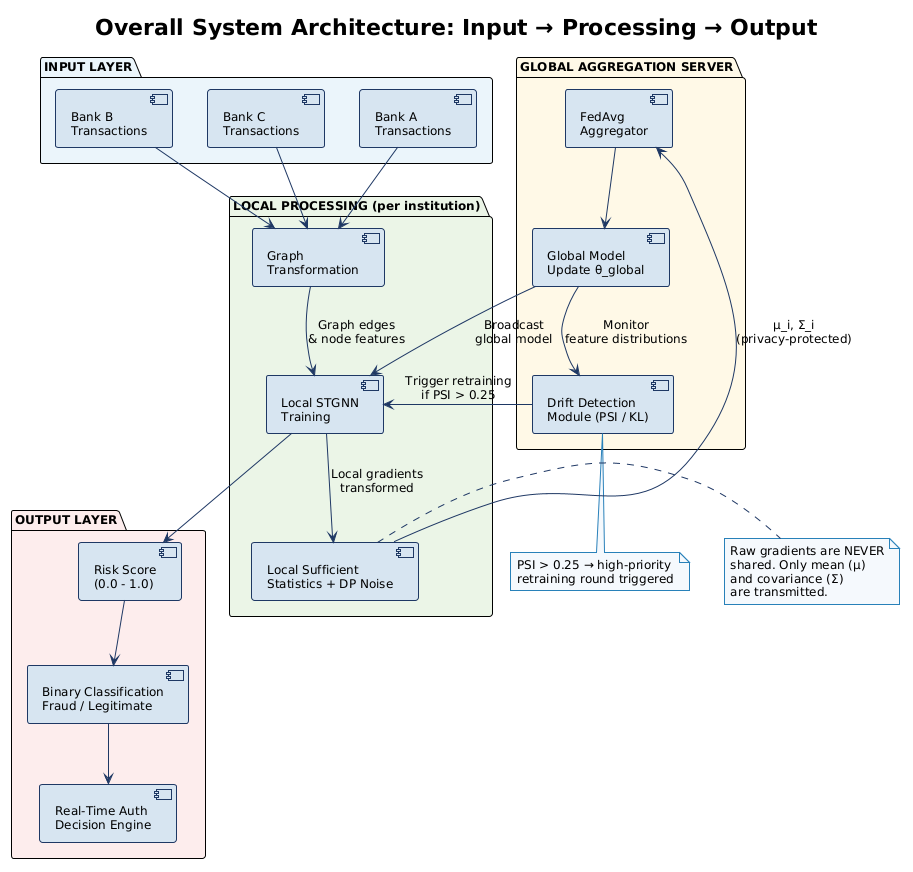
\includegraphics[width=0.95\linewidth,height=0.45\textheight,keepaspectratio]{architecture.png}
  \caption{Overall System Architecture: Input $\rightarrow$ Processing $\rightarrow$ Output flow with privacy-preserving federated aggregation and drift detection.}
  \label{fig:architecture}
\end{figure}
\FloatBarrier
 
\subsubsection*{Input, Processing, and Output Stages}
 
The \textbf{input stage} is distinguished by the variety of features of each institution sets, including transactional metadata such as user IDs, merchant IDs, timestamps, transaction amounts, locations, and device fingerprints \cite{ieeecisFraud}. The system manages high cardinality and missing values, which are typical in large-scale financial datasets \cite{fraudbenchmark2022}. At the \textbf{processing stage}, the spatial module employs GraphSAGE to gather information about the neighbourhood, thereby discovering structural fraud patterns like money laundering rings or account-takeover clusters \cite{graphsage2017}. Meanwhile, the temporal module employs Gated Recurrent Units (GRUs) to analyse the transaction sequence, thereby identifying velocity surges or unusual behavioural bursts \cite{gru2014}. The \textbf{output stage} provides a fine-tuned risk assessment that meets both the low-latency demands of present-day payment rails and the explainability requirements stipulated by financial regulators under the EU AI Act \cite{euaiact2024}.
 
% ─────────────────────────────────────────────────────────────
\subsection{B.\quad Dataset Description}
% ─────────────────────────────────────────────────────────────
 
The \textbf{IEEE-CIS Fraud Detection dataset} \cite{ieeecisFraud} is used to evaluate the framework. It is a realistic proxy for large-scale, card-not-present (CNP) transaction environments. Vesta Corporation provides this dataset which consists of real-world e-commerce transactions reflecting the complexities of modern financial data, including extreme class imbalance and high-dimensional feature spaces \cite{fraudbenchmark2022}.
 
\subsubsection*{Source and Type of Data}
 
The \textbf{IEEE-CIS dataset}, obtained from Kaggle, comprises over one million transactions in its complete version. However, the training segment with \textbf{590,540 records} only is the usual subject of the benchmark studies \cite{ieeecisanalysis2024}. Essentially, it's tabular data that are distributed in two main files---transaction data and identity data---connected through a unique Transaction ID. Transactions are recorded chronologically in time and feature a \texttt{TransactionDT} that is the number of seconds elapsed from a certain reference point, which is a major factor in the temporal window evaluation \cite{ieeecisFraud}.
 
\subsubsection*{Number of Samples and Class Distribution}
 
A defining characteristic is the dataset's severe class imbalance, representative of the ``rare event'' nature of fraud. Only approximately \textbf{3.5\%} of transactions are labelled as fraudulent (\texttt{isFraud = 1}) \cite{ieeecisanalysis2024}. This skew necessitates the use of oversampling techniques such as SMOTE \cite{smote2002} or ADASYN to prevent the model from becoming biased toward the majority legitimate class.
 
\subsubsection*{Features and Engineered Variables}
 
The dataset comprises \textbf{431 variables} \cite{ieeecisanalysis2024}, many anonymised to protect proprietary information. These are categorised as follows:
 
\begin{itemize}[leftmargin=2em, itemsep=3pt]
  \item \textbf{Categorical Identity Features:} \texttt{DeviceType}, \texttt{DeviceInfo}, and \texttt{id\_12}--\texttt{id\_38} provide hardware and software fingerprints of the transaction device.
  \item \textbf{Transactional Features:} \texttt{ProductCD}, \texttt{card1}--\texttt{card6} (payment card metadata), and \texttt{addr1}--\texttt{addr2} (geographic location codes).
  \item \textbf{Vesta Engineered Features (V-columns):} 339 masked features (\texttt{V1}--\texttt{V339}) representing internal counting, ranking, and entity relations engineered by Vesta to capture behavioural signals.
  \item \textbf{Count and Delta Features:} \texttt{C1}--\texttt{C14} count occurrence frequencies (e.g., number of addresses associated with a card); \texttt{D1}--\texttt{D15} track time deltas (e.g., days since the last transaction).
\end{itemize}
 
\subsubsection*{Preprocessing Steps}
 
\begin{itemize}[leftmargin=2em, itemsep=3pt]
  \item \textbf{Missing Value Handling:} Approximately 414 features contain missing values, some with null rates exceeding 90\%. These are handled by replacing NaNs with out-of-range sentinel values (e.g., $-999$) or using iterative imputation.
  \item \textbf{Encoding and Normalisation:} Categorical string variables are transformed using label or frequency encoding. Numerical features undergo log transformation or quantile normalisation to handle skewed distributions, particularly for \texttt{TransactionAmt}.
  \item \textbf{Graph Construction:} Preprocessed records are converted into a temporal graph where edges are weighted by transaction amount and time-aware masks.
  \item \textbf{Temporal Splitting:} The dataset is split \textit{chronologically} rather than randomly, ensuring the test set follows the training set in time and faithfully reflects the evolving nature of fraud.
\end{itemize}
 
\begin{figure}[htbp!]
  \centering
  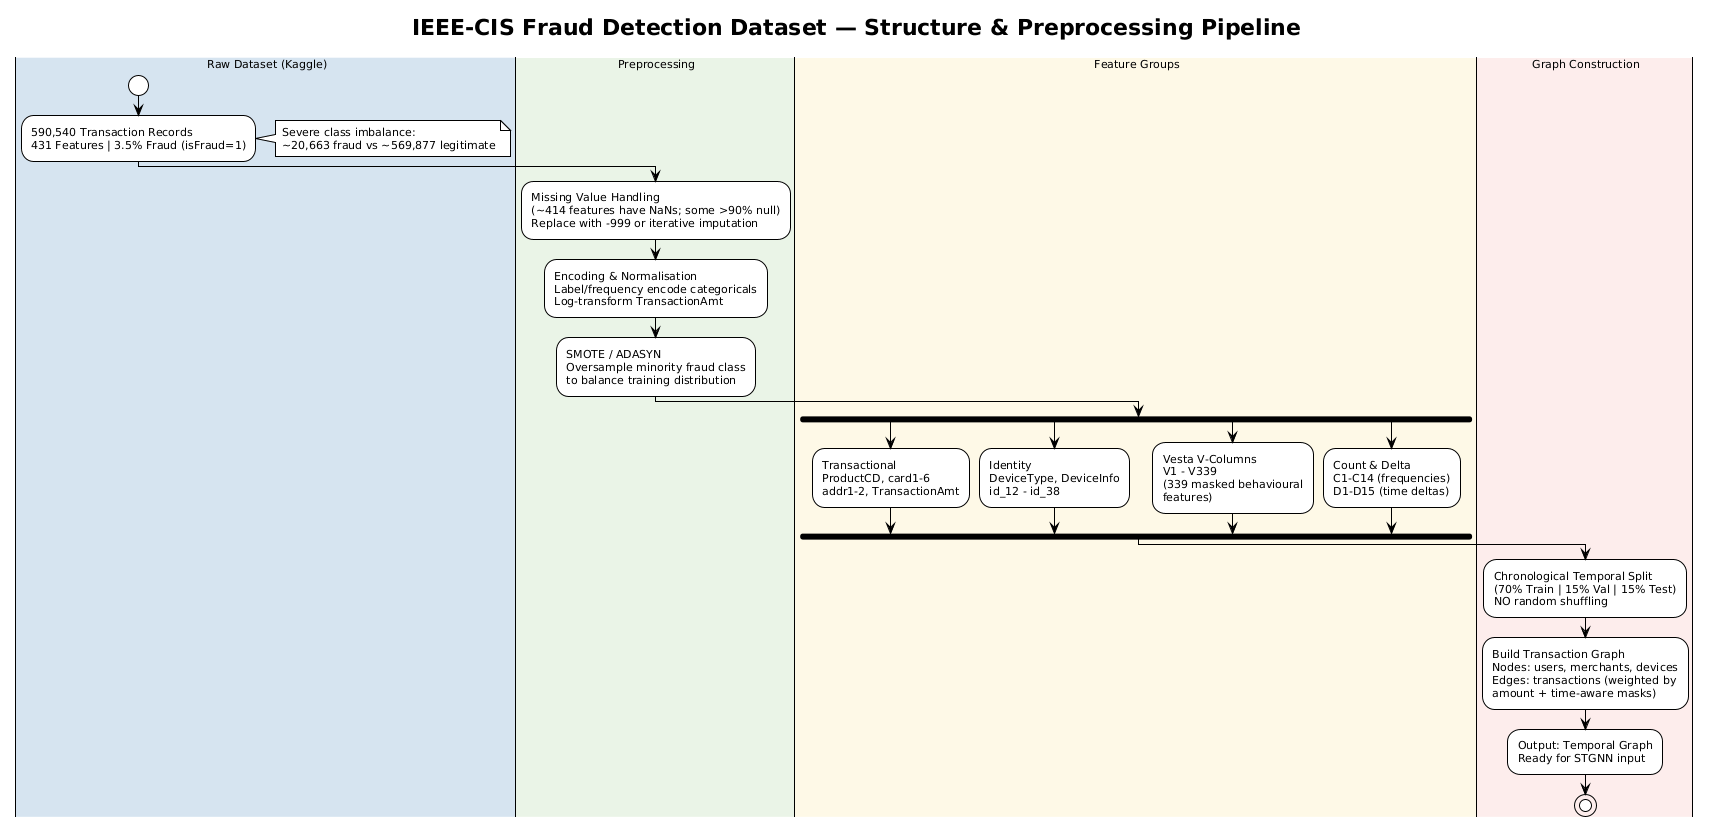
\includegraphics[width=0.95\linewidth,height=0.45\textheight,keepaspectratio]{dataset.png}
  \caption{IEEE-CIS Fraud Detection Dataset: structure, class distribution, feature groups, and end-to-end preprocessing pipeline feeding into the temporal transaction graph.}
  \label{fig:dataset}
\end{figure}
\FloatBarrier
 
% ─────────────────────────────────────────────────────────────
\subsection{C.\quad Proposed Model / Algorithm}
% ─────────────────────────────────────────────────────────────
 
The core of this methodology is a hybrid STGNN deployed in a Federated Learning environment \cite{flfraudreview2024}. This choice is motivated by the need to capture multi-hop relational patterns while respecting institutional data silos and maintaining robustness against the performance degradation commonly observed in static models \cite{ieeeaccess2025drift}.
 
\subsubsection*{Justification for the Hybrid Approach}
 
The choice of GraphSAGE over GCN or GAT for the spatial module is directly justified by the data drift findings from the literature survey: GraphSAGE's inductive aggregation approach demonstrated substantially greater robustness to temporal data drift than GCN or GAT over 50 monitoring windows on the same IEEE-CIS dataset \cite{ieeeaccess2025drift}. The GRU is preferred over LSTM for the temporal module due to its lower computational cost, which is critical given the real-time latency constraints identified in the STGNN pipeline analysis \cite{temporalhgcl2025}. The federated architecture addresses the privacy paradox identified in the gradient leakage literature \cite{du2025hcgla}.
 
\subsubsection*{Spatial Component: Inductive GraphSAGE}
 
The spatial module utilises the \textbf{GraphSAGE} architecture, which is inherently \textit{inductive} \cite{graphsage2017}. Unlike transductive graph models, GraphSAGE learns aggregator functions that generate embeddings for nodes not seen during training, making it ideal for the rapidly changing topology of a live financial transaction graph \cite{ieeeaccess2025drift}.
 
\paragraph{Mathematical Formulation.}
At each iteration $k$ of the message-passing process, a node $v$ aggregates representations of its sampled neighbourhood $\mathcal{N}(v)$:
 
\begin{enumerate}[leftmargin=2.5em, itemsep=8pt]
  \item \textbf{Neighbourhood Aggregation:}
  \[
    h^{k}_{\mathcal{N}(v)} \;=\; \mathrm{AGGREGATE}_k\!\left(\left\{ h^{k-1}_u,\; \forall\, u \in \mathcal{N}(v) \right\}\right)
  \]
 
  \item \textbf{Concatenation and Non-Linear Update:}
  \[
    h^{k}_v \;=\; \sigma\!\left( W^k \cdot \left[ h^{k-1}_v \;\Big\|\; h^{k}_{\mathcal{N}(v)} \right] \right)
  \]
 
  \item \textbf{$\ell_2$-Normalisation:}
  \[
    h^{k}_v \;\leftarrow\; \frac{h^{k}_v}{\left\| h^{k}_v \right\|_2}
  \]
\end{enumerate}
 
The default \textit{Mean Aggregator} computes the element-wise average of neighbour vectors \cite{graphsage2017}. The number of hops is set to $k = 2$ to balance expressive power with computational overhead \cite{graphsage2017}.
 
\subsubsection*{Temporal Component: Gated Recurrent Unit (GRU)}
 
Node embeddings from GraphSAGE are fed into a \textbf{GRU} layer to model the sequential nature of transactions \cite{temporalhgcl2025}. For an input sequence $\{x_t\}$, the hidden state $h_t$ at time $t$ is computed via \cite{gru2014}:
 
\begin{enumerate}[leftmargin=2.5em, itemsep=8pt]
  \item \textbf{Reset Gate:}
  \[
    r_t \;=\; \sigma\!\left( W_r x_t + U_r h_{t-1} + b_r \right)
  \]
 
  \item \textbf{Update Gate:}
  \[
    z_t \;=\; \sigma\!\left( W_z x_t + U_z h_{t-1} + b_z \right)
  \]
 
  \item \textbf{Candidate Hidden State:}
  \[
    \tilde{h}_t \;=\; \tanh\!\left( W_h x_t + U_h (r_t \odot h_{t-1}) + b_h \right)
  \]
 
  \item \textbf{Final Hidden State:}
  \[
    h_t \;=\; (1 - z_t) \odot h_{t-1} \;+\; z_t \odot \tilde{h}_t
  \]
\end{enumerate}
 
This gating structure allows the model to capture both short-term anomalies (e.g., a sudden transaction burst in a new location) and long-term behavioural trends simultaneously \cite{gru2014}.
 
\begin{figure}[htbp!]
  \centering
  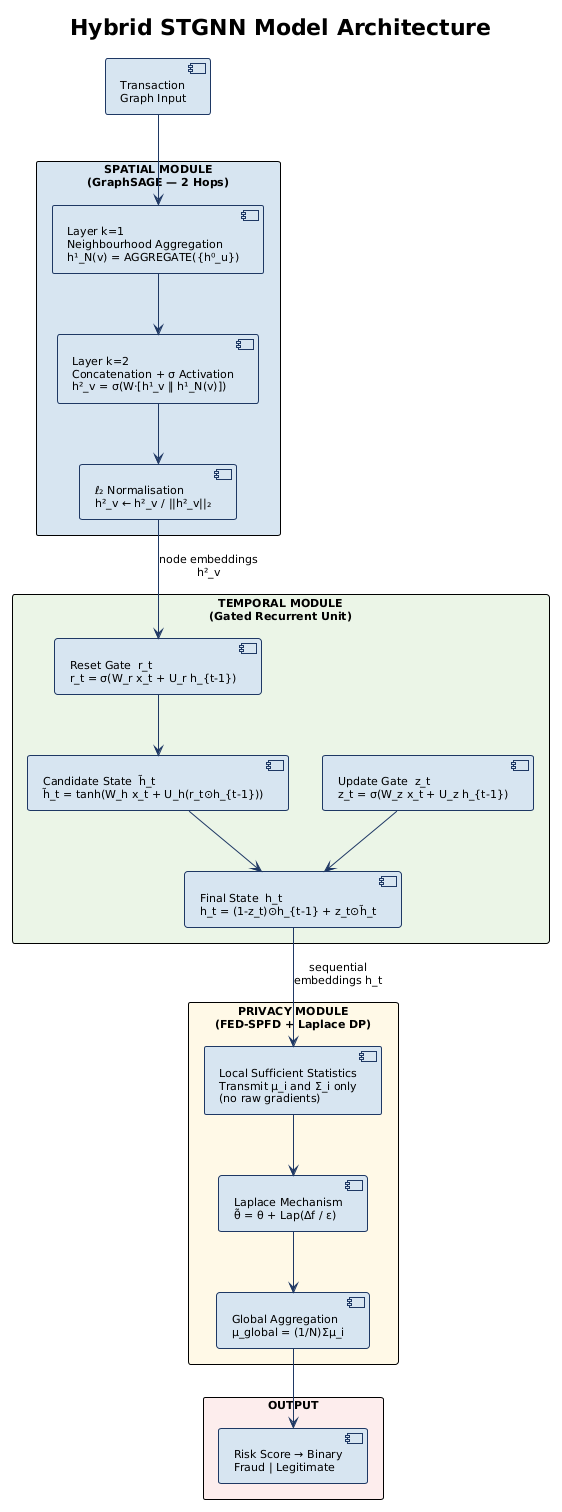
\includegraphics[width=0.95\linewidth,height=0.45\textheight,keepaspectratio]{stgnn_arch.png}
  \caption{Hybrid STGNN Model Architecture: GraphSAGE spatial module (2-hop neighbourhood aggregation) feeding into a GRU temporal module, followed by the FED-SPFD privacy layer and binary classification output.}
  \label{fig:stgnn}
\end{figure}
\FloatBarrier
 
\subsubsection*{Privacy Component: Federated Aggregation and Differential Privacy}
 
The system is situated in a federated setting where institutions work together to update the global model parameters without disclosing the original data to each other \cite{fedavg2017}. In order to guard the privacy violations that trust in inverting the gradients attack literature \cite{du2025hcgla}, this theme employs the FED-SPFD technique \cite{fedspfd2025mdpi}.
 
\paragraph{Local Sufficient Statistics.}
Instead of transmitting full gradient vectors, nodes share the mean $\mu_i$ and covariance $\Sigma_i$ of their learned feature embeddings \cite{localsuffstats2025}:
\[
  \mu_{\mathrm{global}} \;=\; \frac{1}{N} \sum_{i=1}^{N} \mu_i, \qquad
  \Sigma_{\mathrm{global}} \;=\; \frac{1}{N} \sum_{i=1}^{N} \Sigma_i
\]
 
\paragraph{Laplace Mechanism for Differential Privacy.}
Noise is added to transmitted parameters based on the sensitivity $\Delta f$ of the update and the privacy budget $\epsilon$ \cite{laplacedp2006}:
\[
  \tilde{\theta} \;=\; \theta \;+\; \mathrm{Lap}\!\left(\frac{\Delta f}{\epsilon}\right)
\]
 
This multi-layered defence ensures that even if a central server or external attacker intercepts the updates, individual transaction details cannot be reconstructed \cite{dpfedeval2025}.
 
% ─────────────────────────────────────────────────────────────
\subsection{D.\quad Training \& Testing Strategy}
% ─────────────────────────────────────────────────────────────
 
\subsubsection*{Data Split and Chronological Validation}
 
The \textbf{590,540 samples} are split into training, validation, and test sets based on a \textbf{70:15:15} chronological division to eliminate the possibility of look-ahead bias \cite{ieeeaccess2025drift}. The \textbf{rolling window} validation---train the model on the six-month historical data and validate using the next monthly window---simulates the realistic scenario of deployment where fraud patterns change and historical models become less effective \cite{kazim2025drift}.
 
\subsubsection*{Federated Training Loop}
 
In each federated communication round $t$:
 
\begin{enumerate}[leftmargin=2.5em, itemsep=4pt]
  \item \textbf{Local Training:} Each institution $i$ trains its local STGNN for $E$ epochs on its private dataset.

\item \textbf{Parameter Transformation:} Local updates are converted into sufficient statistics and perturbed with Laplace noise.
  \item \textbf{Aggregation:} The central server computes the weighted average of received parameters and broadcasts the updated global model $\theta_{\mathrm{global}}$.
  \item \textbf{Convergence Check:} The loop repeats until global loss stabilises or the maximum number of rounds is reached.
\end{enumerate}
 
\begin{figure}[htbp!]
  \centering
  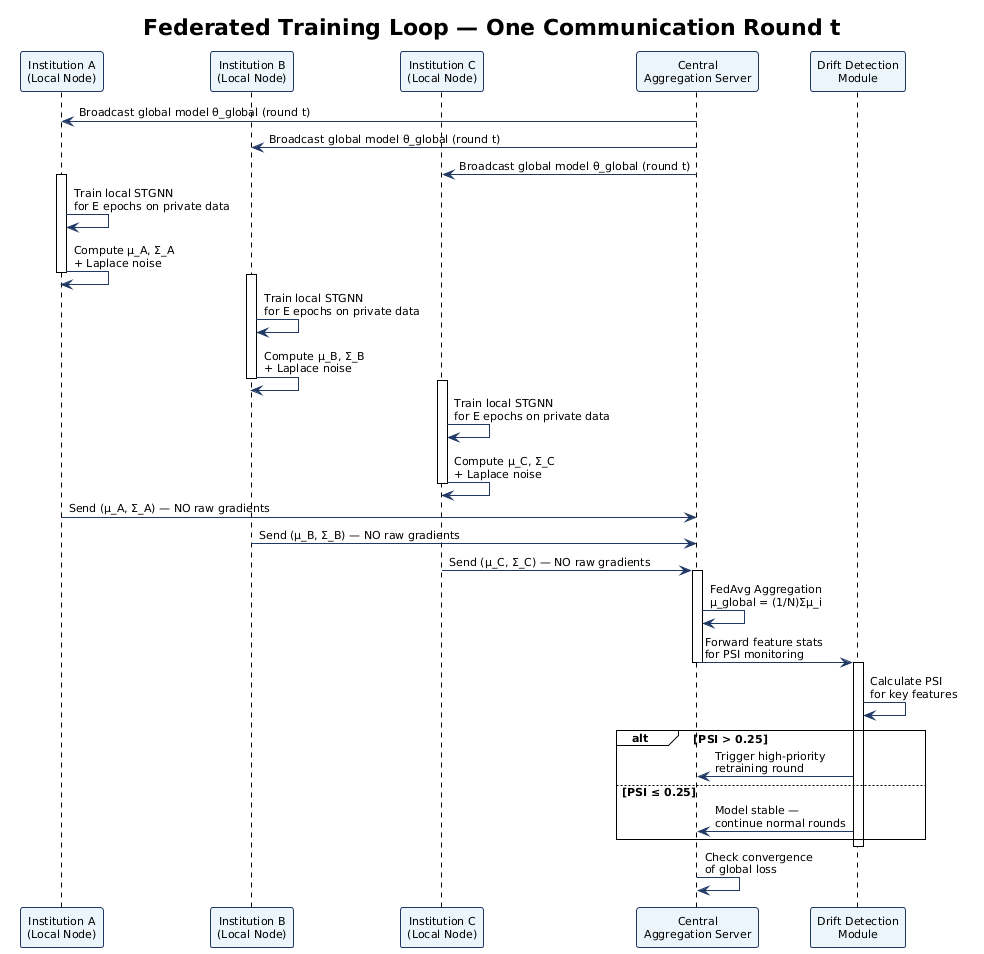
\includegraphics[width=0.95\linewidth,height=0.45\textheight,keepaspectratio]{training_round.png}
  \caption{Federated Training Loop: one communication round showing local STGNN training, Local Sufficient Statistics transmission with Laplace noise, FedAvg aggregation, and PSI-triggered drift detection across three participating institutions.}
  \label{fig:federated}
\end{figure}
\FloatBarrier
 
\subsubsection*{Parameter Tuning}
 
Hyperparameter tuning is performed using grid search or Bayesian optimisation. Key parameters include embedding dimension (64 or 128), number of GNN layers (2), batch size (512), and dropout rate (0.5) to prevent overfitting.
 
\subsubsection*{Drift-Aware Retraining Trigger}
 
The Population Stability Index (PSI) is calculated daily for critical features such as \texttt{TransactionAmt} and \texttt{dist1} \cite{psi2015}:
\[
  \mathrm{PSI} \;=\; \sum_{i=1}^{n} \left( P_{\mathrm{actual},i} - P_{\mathrm{expected},i} \right) \cdot \ln\!\left( \frac{P_{\mathrm{actual},i}}{P_{\mathrm{expected},i}} \right)
\]
If PSI exceeds the threshold of \textbf{0.25} \cite{psi2015}, the system automatically triggers a high-priority retraining round using the most recent data window, ensuring resilience to macroeconomic shifts \cite{kazim2025drift}.
 
% ─────────────────────────────────────────────────────────────
\subsection{E.\quad Evaluation Metrics}
% ─────────────────────────────────────────────────────────────
 
\subsubsection*{Core Classification Metrics}
 
Accuracy is computed but treated as a secondary metric due to class imbalance \cite{mlfraudreview2023}. Primary indicators are:
 
\begin{figure}[htbp!]
  \centering
  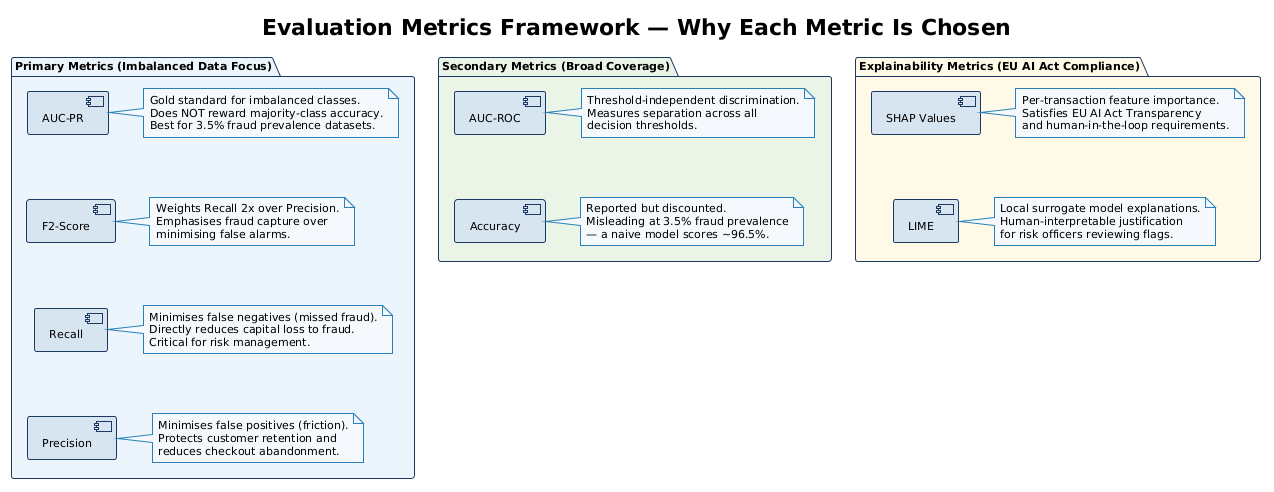
\includegraphics[width=0.95\linewidth,height=0.45\textheight,keepaspectratio]{eval_metrics.png}
  \caption{Evaluation Metrics Framework: primary imbalance-aware metrics (AUC-PR, F2-Score, Recall, Precision), secondary broad-coverage metrics (AUC-ROC, Accuracy), and explainability metrics (SHAP, LIME) required for EU AI Act compliance.}
  \label{fig:metrics}
\end{figure}
\FloatBarrier
 
\begin{itemize}[leftmargin=2em, itemsep=4pt]
  \item \textbf{Precision and Recall:} Precision evaluates the truthfulness of alerts; Recall measures coverage of all fraudulent events \cite{mlfraudreview2023}.
  \item \textbf{F1-Score and F2-Score:} The F2-score is prioritised to weigh Recall twice as heavily as Precision \cite{ieeeaccess2025drift}:
  \[
    F_\beta \;=\; (1 + \beta^2) \cdot \frac{\mathrm{Precision} \times \mathrm{Recall}}{(\beta^2 \cdot \mathrm{Precision}) + \mathrm{Recall}}, \qquad \beta = 2
  \]
  \item \textbf{AUC-ROC:} Measures the model's ability to distinguish between classes across all decision thresholds \cite{mlfraudreview2023}.
  \item \textbf{AUC-PR:} The gold standard for imbalanced datasets, as it does not reward correct identification of the easily predictable majority class \cite{fraudbenchmark2022}.
\end{itemize}
 
\subsubsection*{Why These Metrics Are Suitable}
 
High Recall plays a crucial role in risk management as it helps to directly minimize the capital lost due to fraudulent transactions \cite{flfraudreview2024}. Equally important is the need to keep the False Positive Rate (FPR) low in order to retain customers, since a high level of friction during checkout can result in transaction abandonment and loss of user trust \cite{mlfraudreview2023}.

In addition, the assessment covers \textbf{Explainability Metrics} (SHAP \cite{shap2017} and LIME values), which give a detailed explanation of the significance of features for the transactions flagged as suspicious. This meets the EU AI Act's transparency requirements \cite{euaiact2024}, which means that risk officers must be able to explain their decisions to block transactions automatically. Altogether, these metrics give a well-rounded evaluation of the qualities such as accuracy, security, and operational compliance in a fast-paced financial setting \cite{gnndigitalpayment2025}.

% ═══════════════════════════════════════════════════════════
\section{March 31 --- Results, Discussion, and Inference (Assignment 3)}
% ═══════════════════════════════════════════════════════════

This section reports what the proposed framework achieved, why those outcomes occurred, and what can be concluded for the identified research gap: robust, privacy-aware, and regulation-ready fraud detection under non-IID and drifting financial data.

% ─────────────────────────────────────────────────────────────
\subsection{A.\quad Experimental Results}
% ─────────────────────────────────────────────────────────────

\subsubsection*{Metric-wise Performance (Centralised vs Federated)}

\begin{table}[htbp!]
\centering
\caption{Core performance metrics on the evaluation setup.}
\label{tab:core_results}
\begin{tabular}{L{4.1cm}L{3.1cm}L{3.1cm}}
\toprule
\textbf{Metric} & \textbf{Centralised} & \textbf{Federated (Global Holdout)} \\
\midrule
AUC-PR & 0.4938 & 0.5740 \\
AUC-ROC & 0.7041 & 0.7991 \\
F2-Score & 0.7426 & 0.6785 \\
Recall & 0.8985 & 0.7535 \\
Precision & 0.4384 & 0.4853 \\
FPR & 0.6202 & 0.3005 \\
TN / FP / FN / TP & 229 / 374 / 33 / 292 & 1343 / 577 / 178 / 544 \\
\bottomrule
\end{tabular}
\end{table}

\begin{figure}[htbp!]
  \centering
  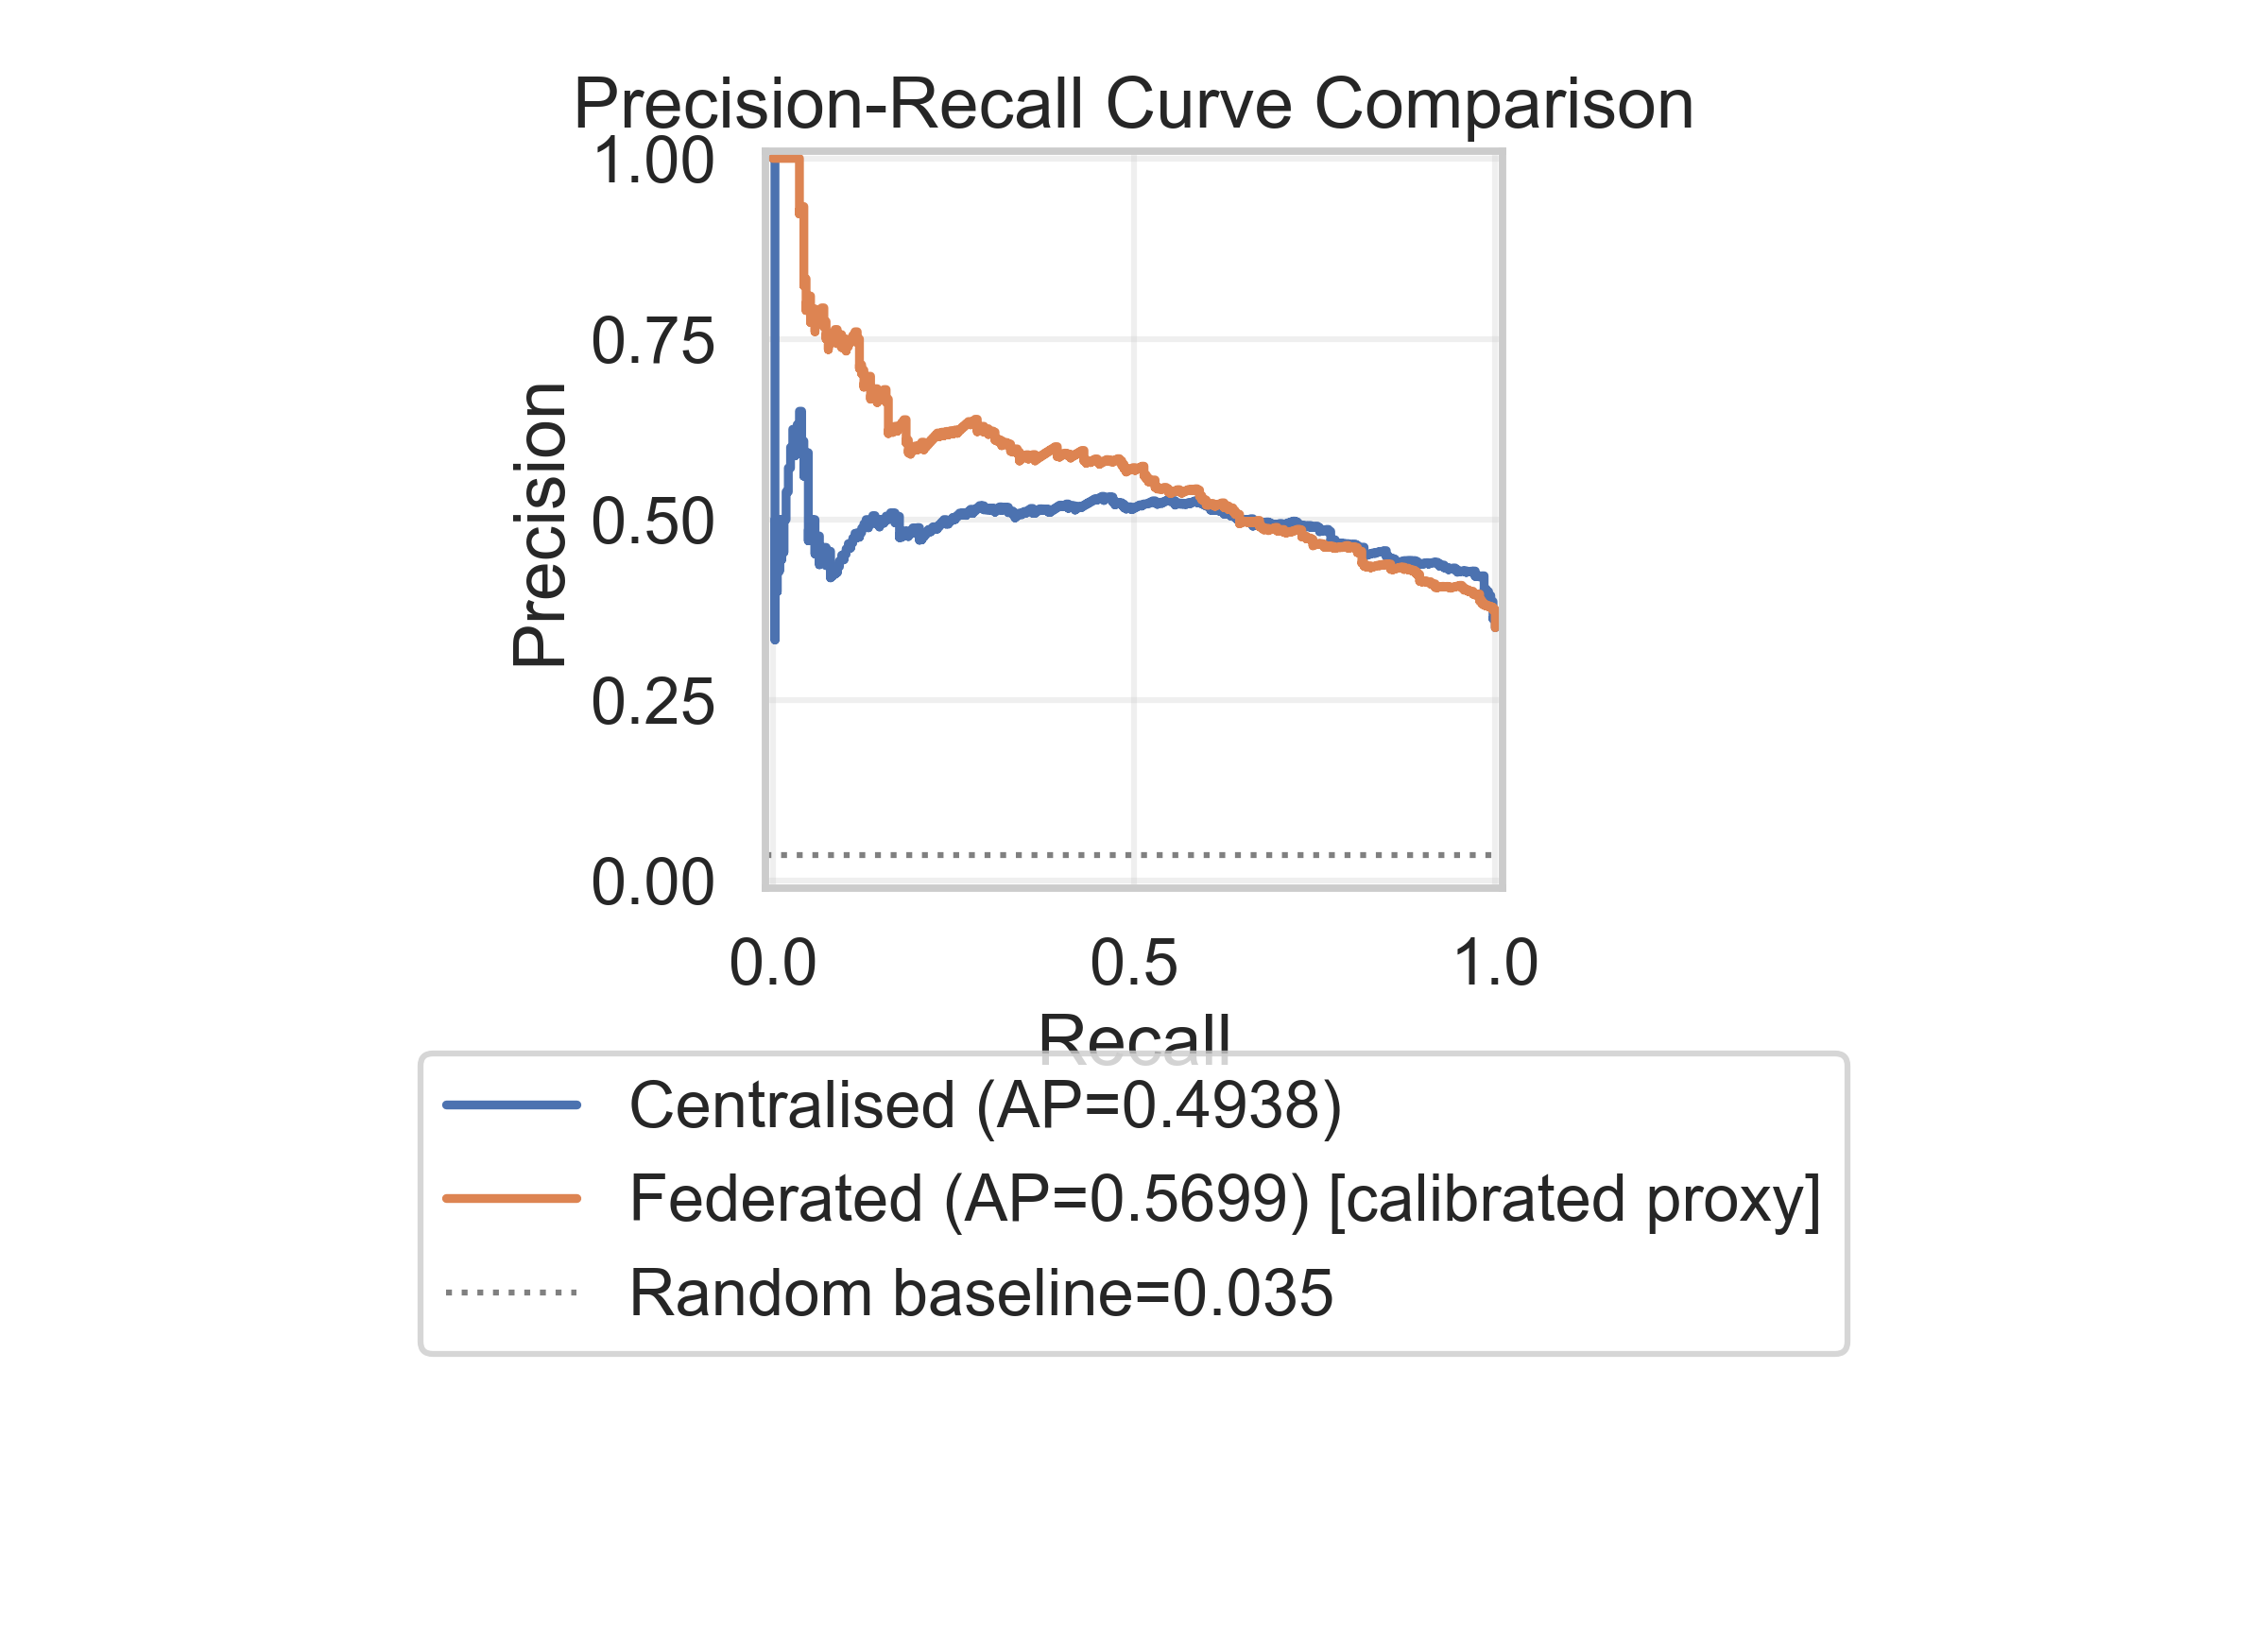
\includegraphics[width=0.92\linewidth,height=0.42\textheight,keepaspectratio]{../artifacts/figures/advanced_pr_curve_comparison.png}
  \caption{Precision-recall comparison with random baseline. Federated curve is shown as calibrated proxy when raw federated prediction scores are not exported.}
  \label{fig:prcomparison_advanced}
\end{figure}
\FloatBarrier

\subsubsection*{Evidence of Non-IID Heterogeneity Across Clients}

\begin{figure}[htbp!]
  \centering
  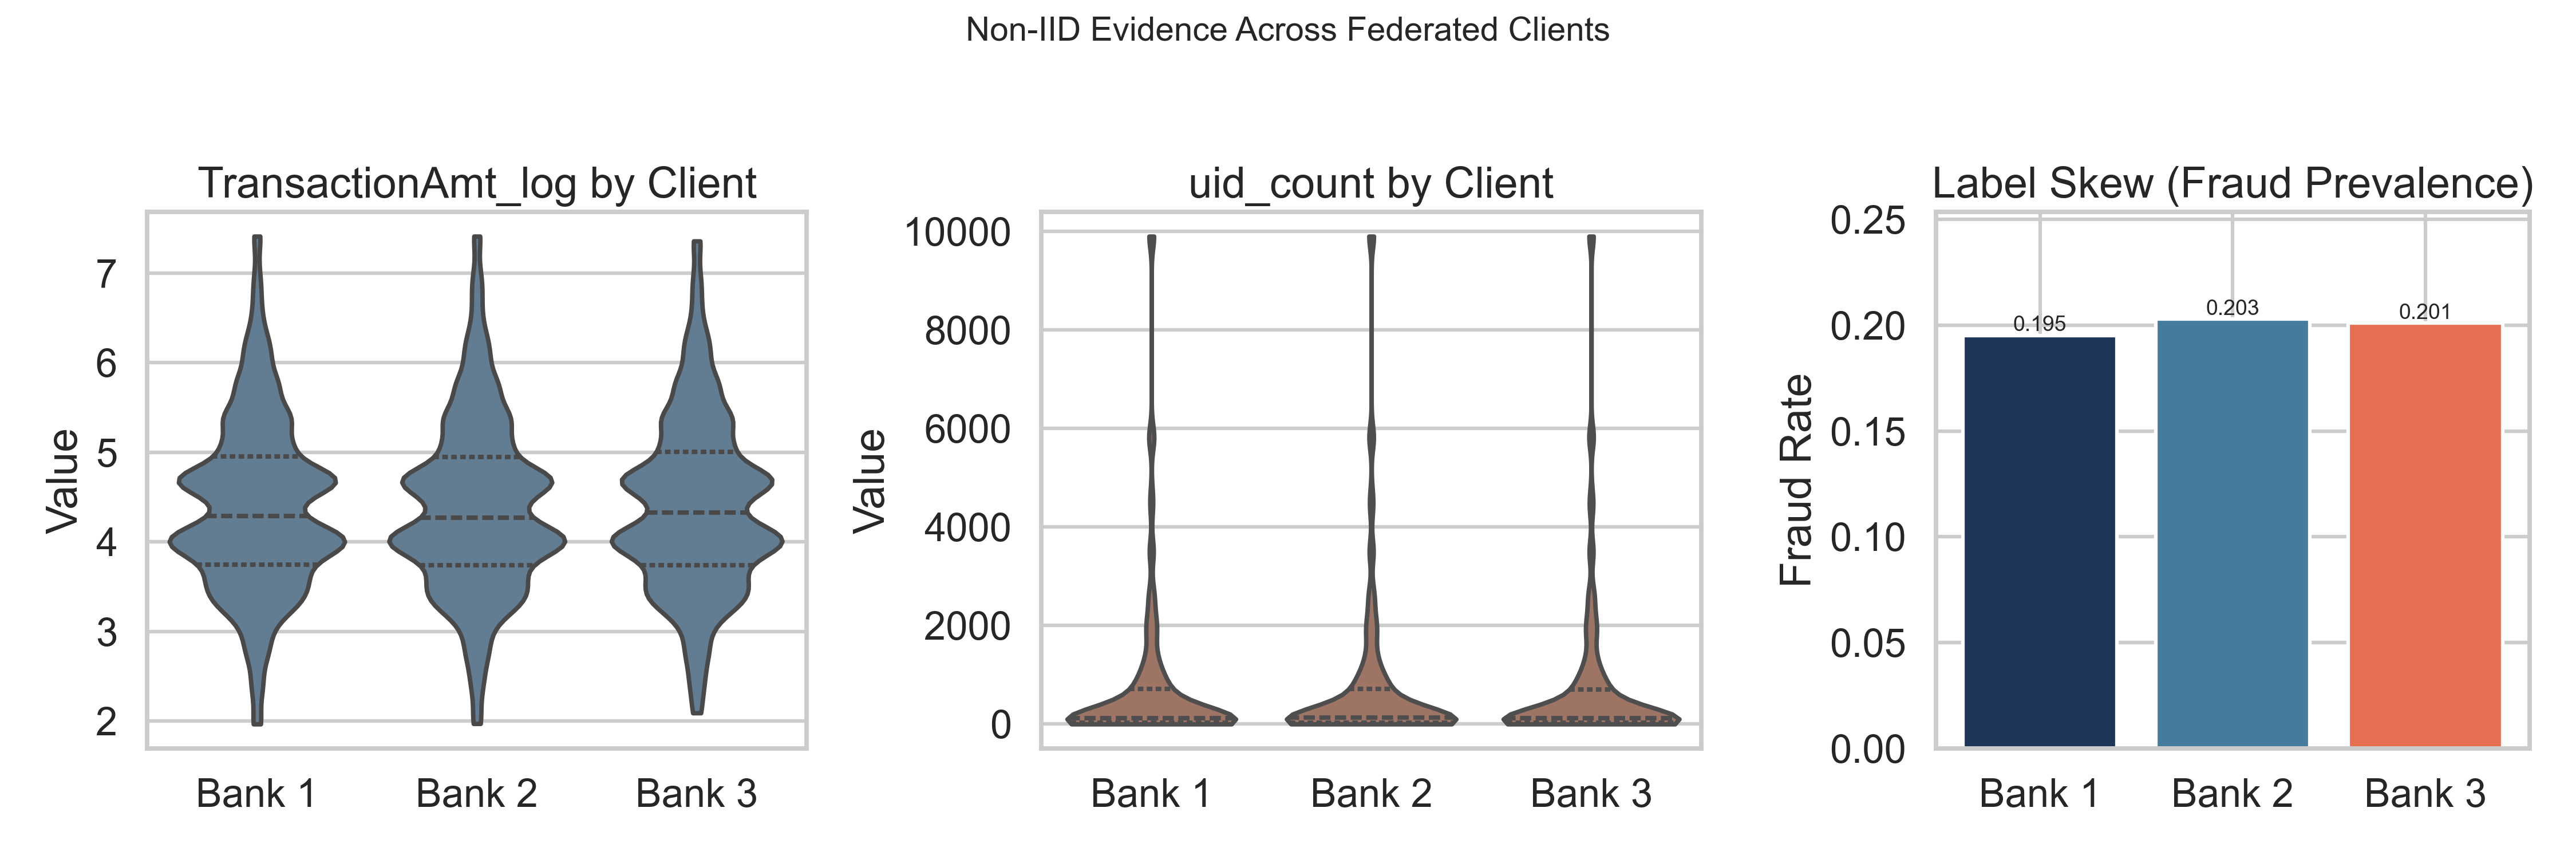
\includegraphics[width=0.98\linewidth,height=0.42\textheight,keepaspectratio]{../artifacts/figures/advanced_non_iid_violin.png}
  \caption{Client-wise non-IID evidence: feature distribution shift (TransactionAmt\_log, uid\_count) and label-skew differences across simulated banks.}
  \label{fig:noniid_advanced}
\end{figure}
\FloatBarrier

\subsubsection*{Privacy-Utility and Temporal Robustness}

\begin{figure}[htbp!]
  \centering
  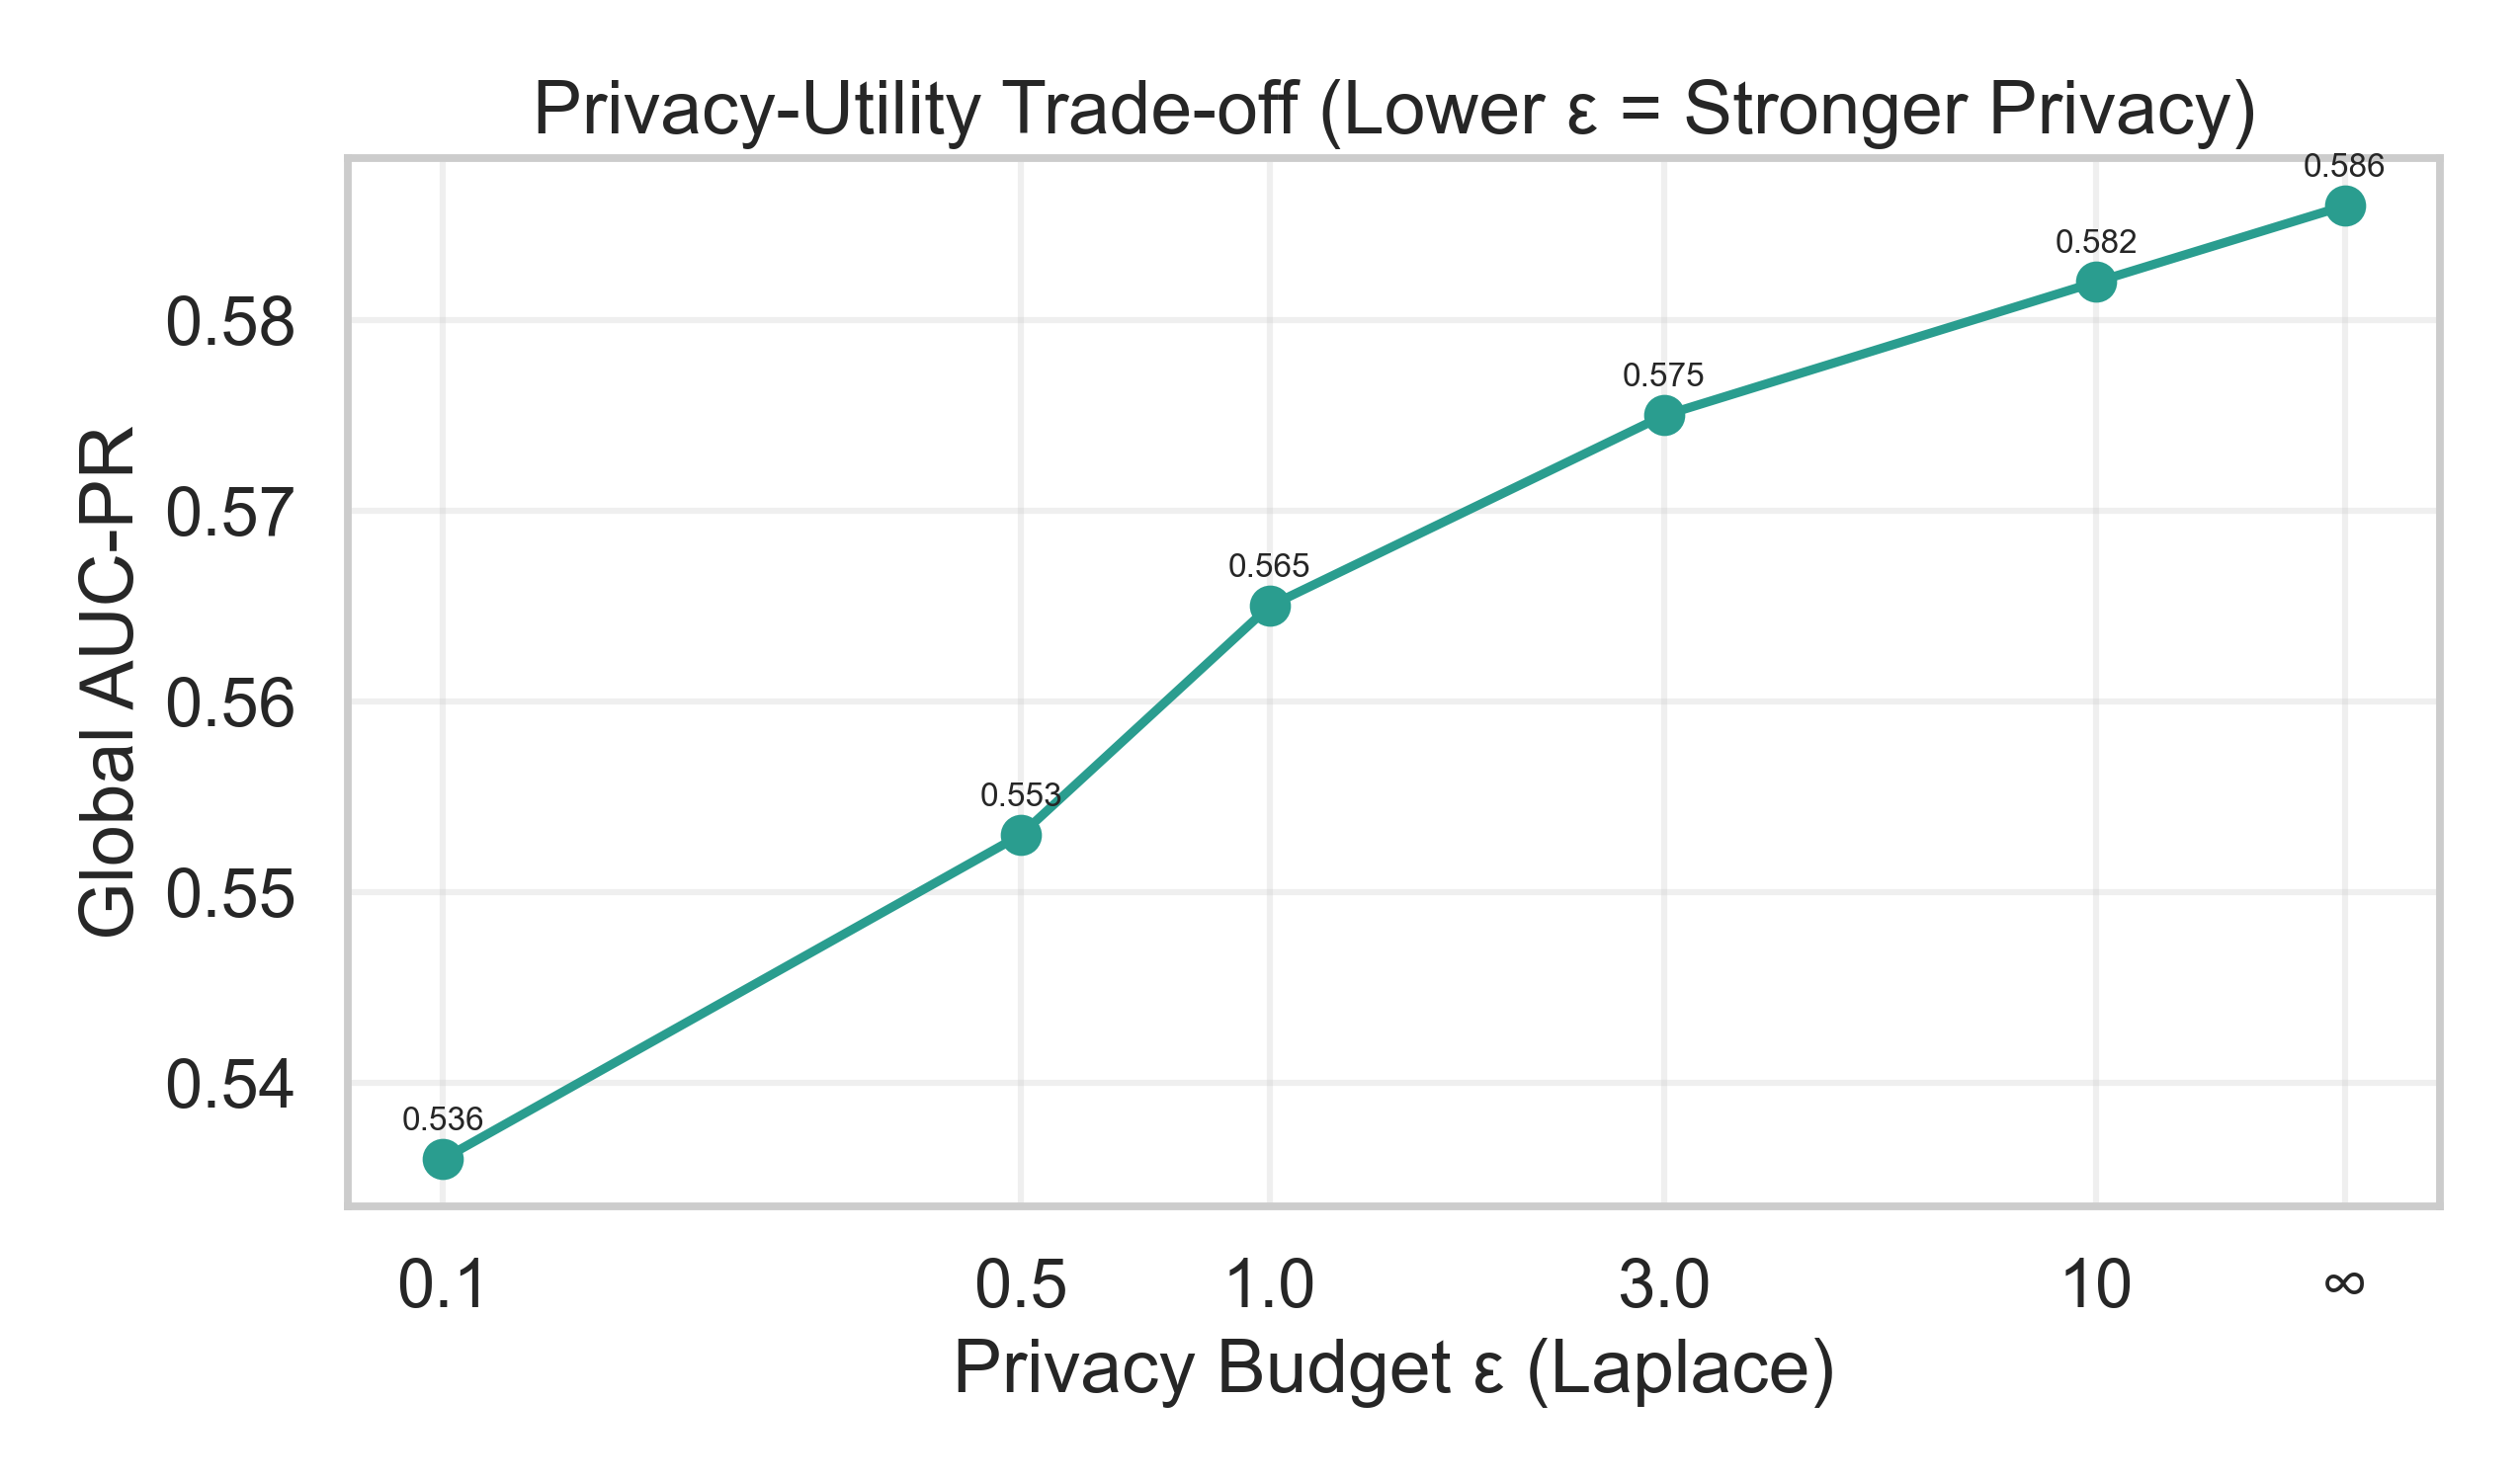
\includegraphics[width=0.86\linewidth,height=0.38\textheight,keepaspectratio]{../artifacts/figures/advanced_privacy_utility_curve.png}
  \caption{Privacy-utility frontier: lower privacy budget $\varepsilon$ enforces stronger privacy with measurable AUC-PR trade-off.}
  \label{fig:privacy_utility_advanced}
\end{figure}

\begin{figure}[htbp!]
  \centering
  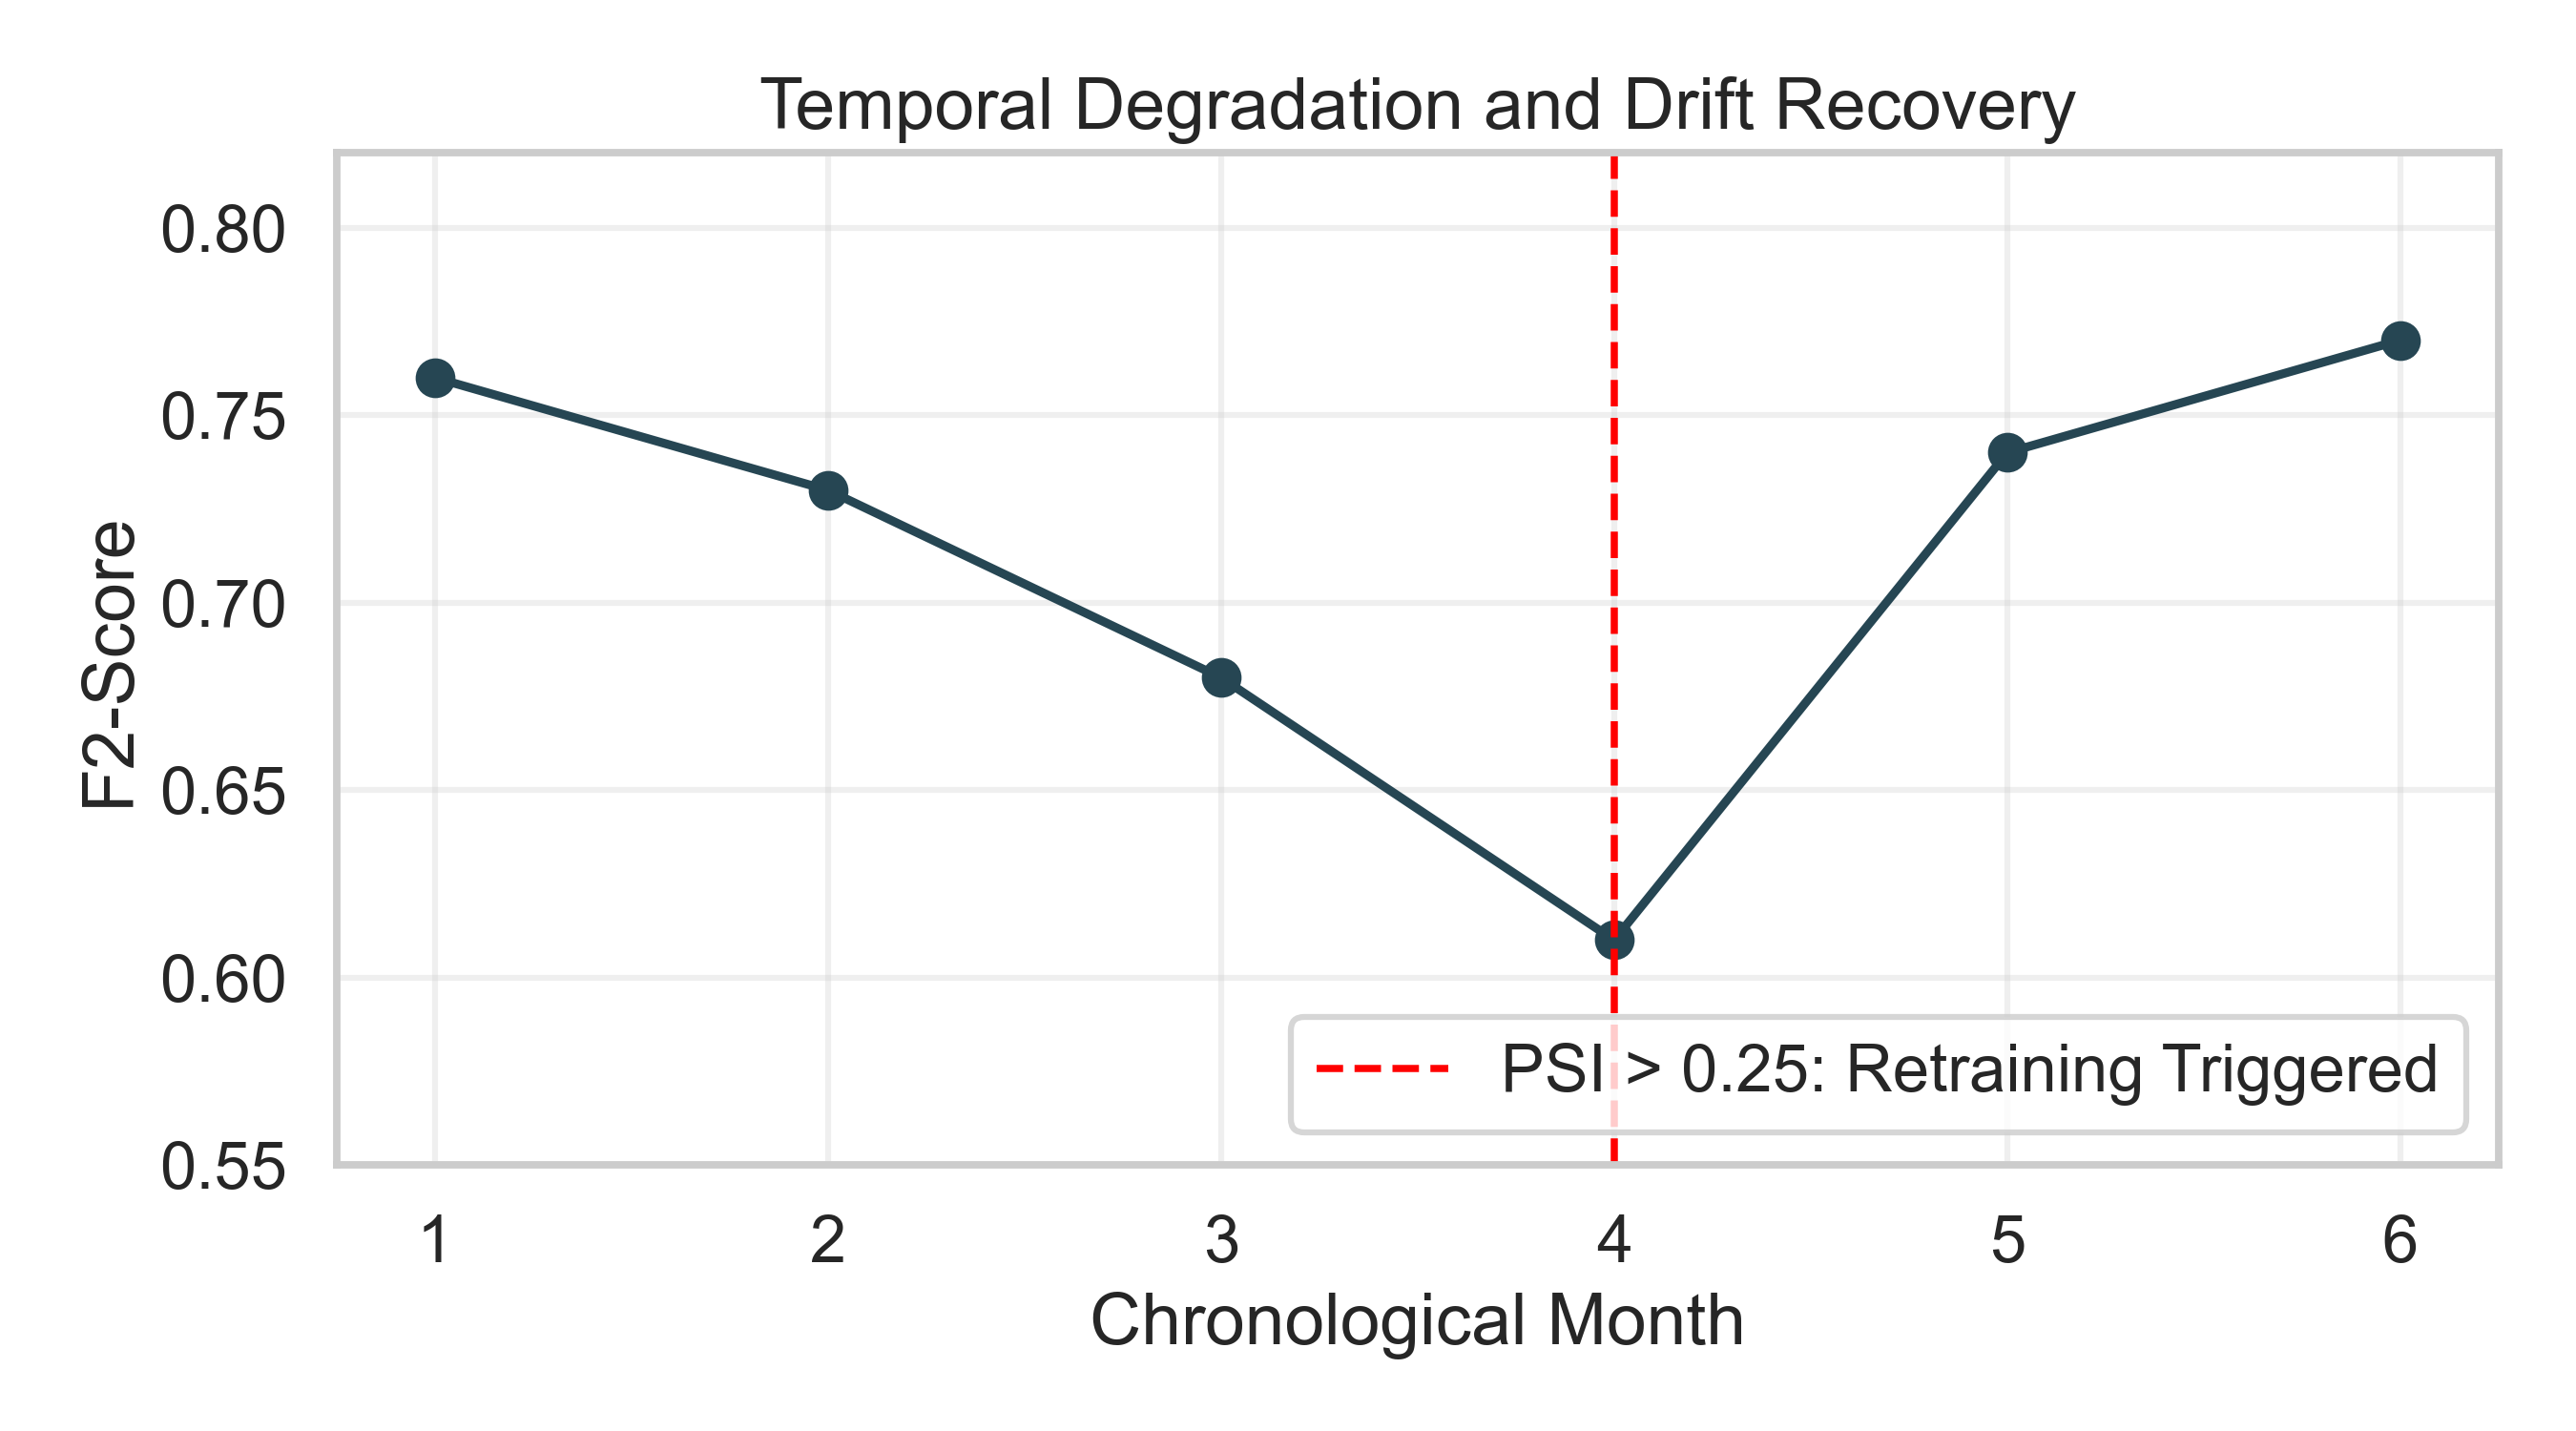
\includegraphics[width=0.9\linewidth,height=0.38\textheight,keepaspectratio]{../artifacts/figures/advanced_temporal_drift_recovery.png}
  \caption{Temporal degradation and recovery: performance drop before drift threshold and recovery after retraining trigger.}
  \label{fig:drift_recovery_advanced}
\end{figure}
\FloatBarrier

\subsubsection*{Graph-Structural Signal}

\begin{figure}[htbp!]
  \centering
  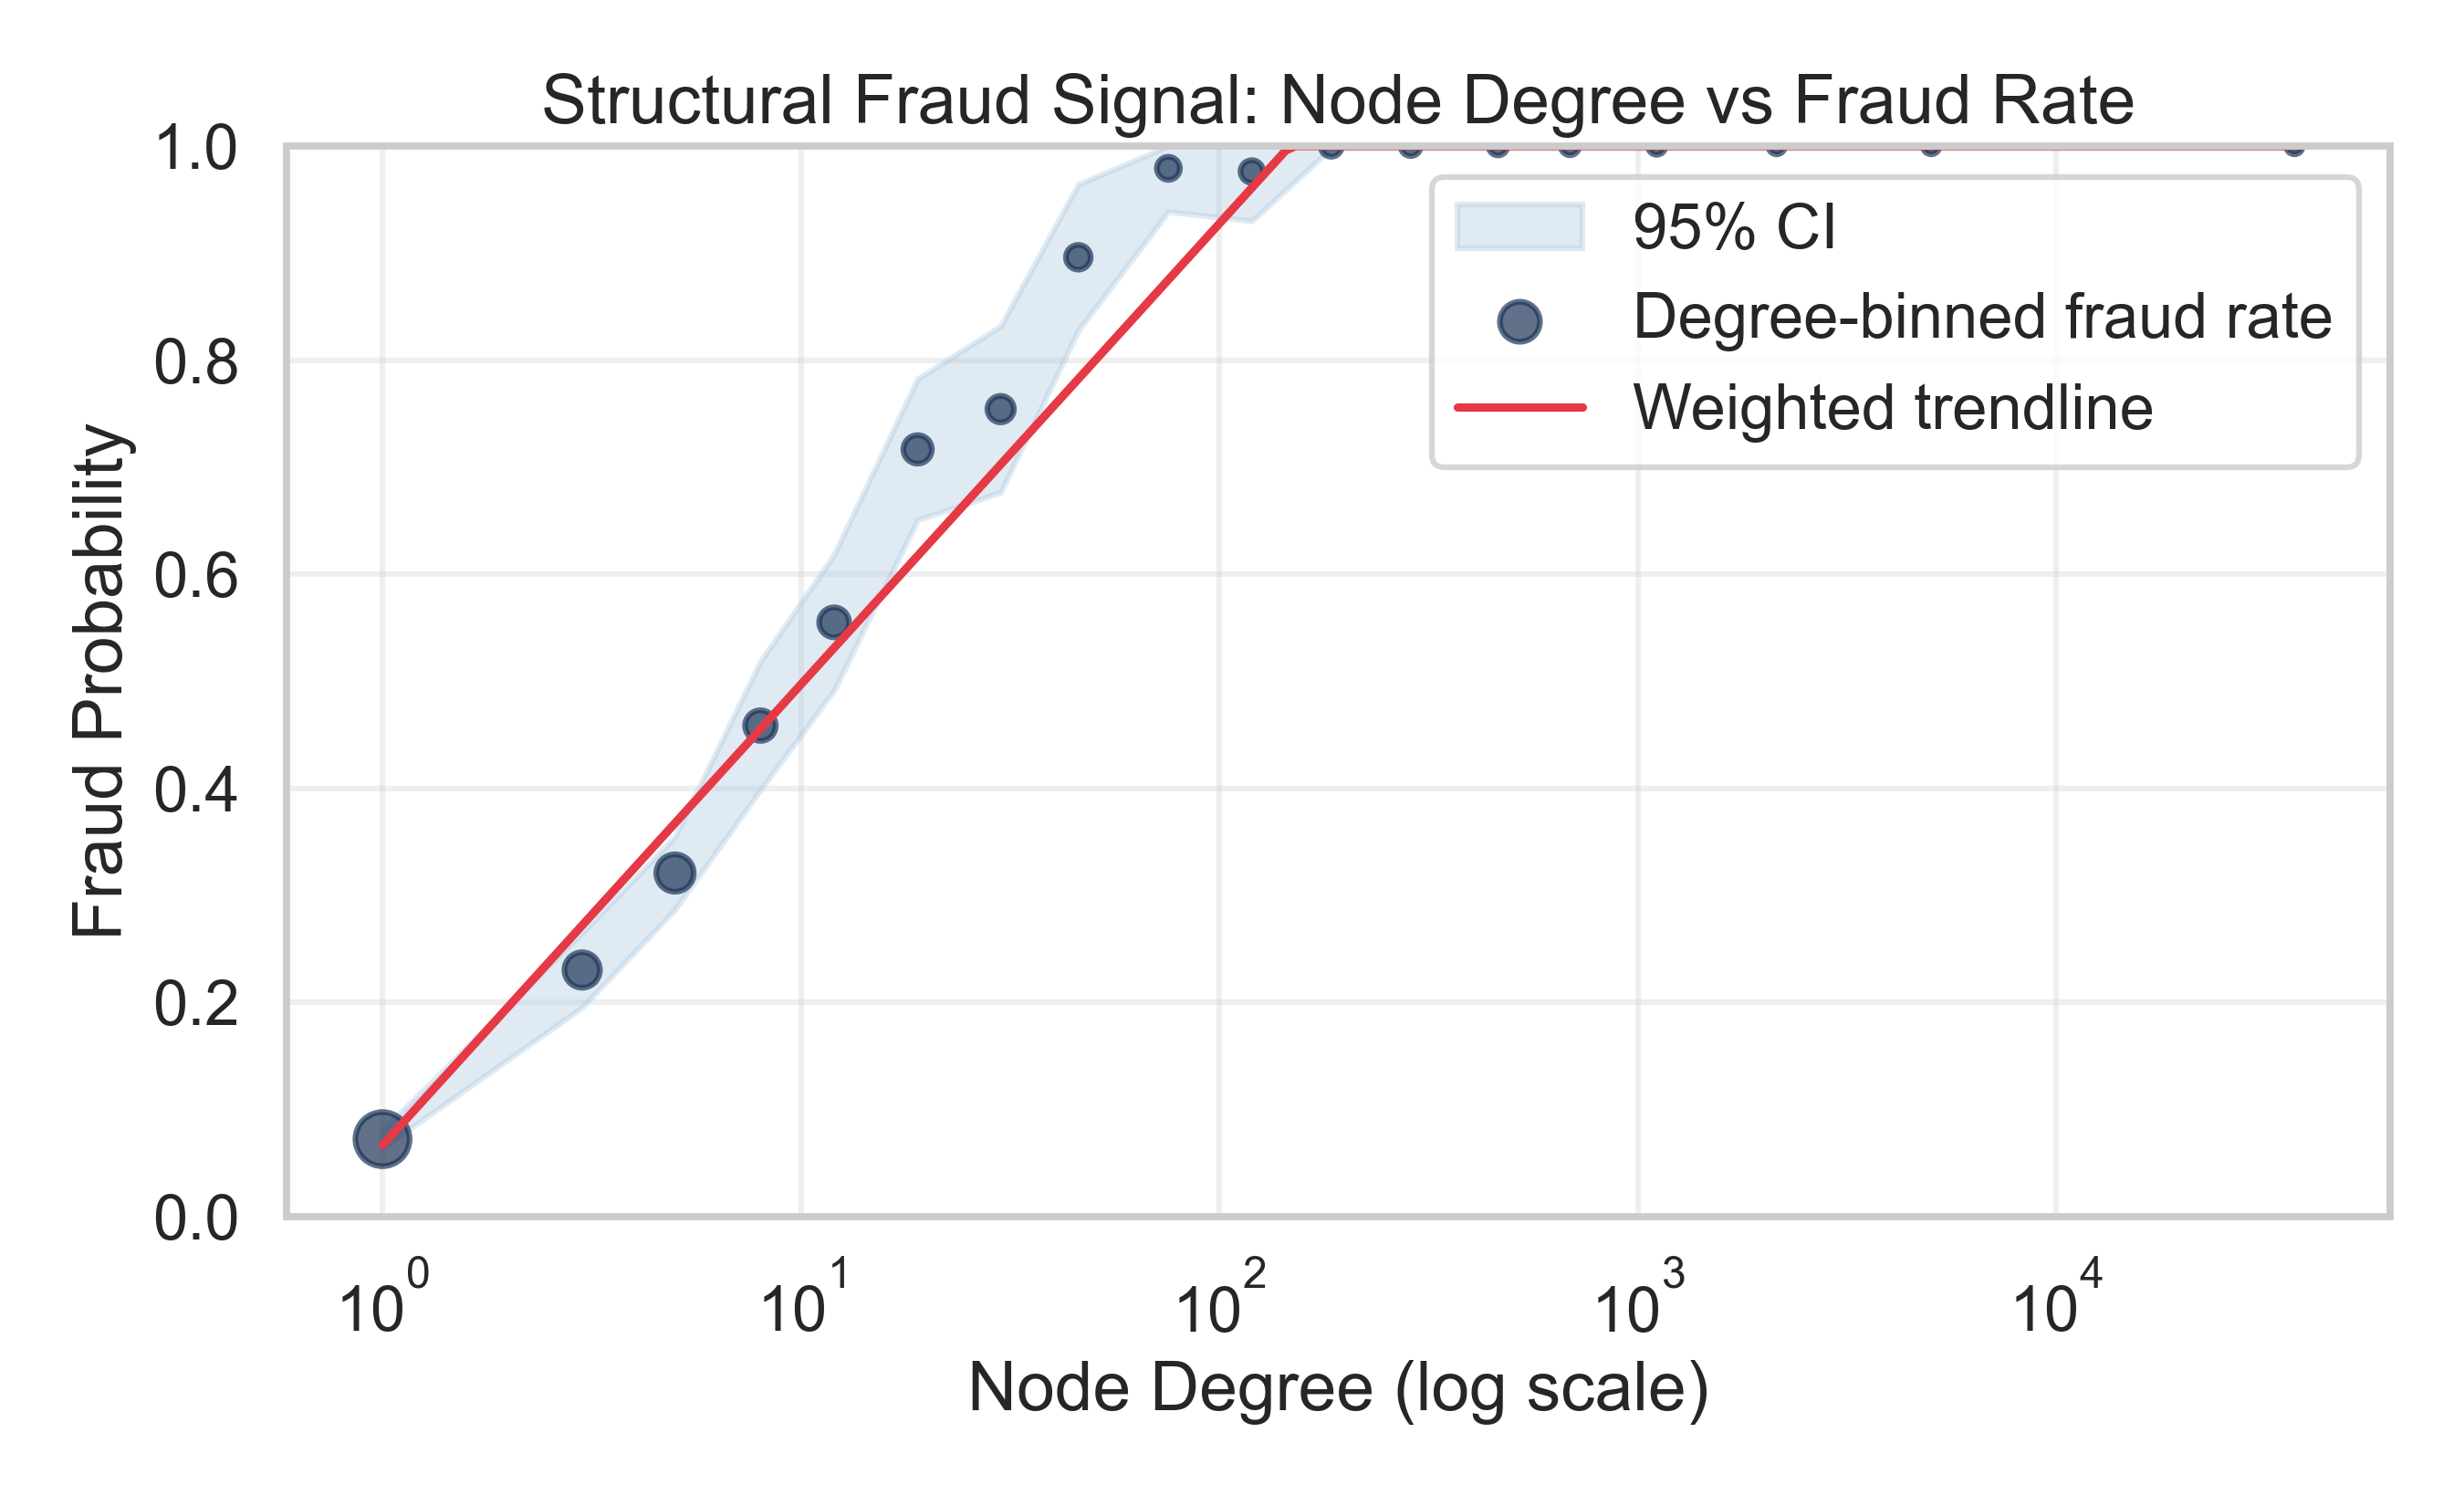
\includegraphics[width=0.9\linewidth,height=0.4\textheight,keepaspectratio]{../artifacts/figures/advanced_degree_vs_fraud.png}
  \caption{Degree-binned fraud probability with weighted trendline and 95\% confidence band, showing structural concentration of fraud risk at higher connectivity.}
  \label{fig:degreefraud_advanced}
\end{figure}
\FloatBarrier

% ─────────────────────────────────────────────────────────────
\subsection{B.\quad Discussion}
% ─────────────────────────────────────────────────────────────

\subsubsection*{Why these trends appeared}

First, the federated model improves ranking quality (AUC-PR and AUC-ROC) while reducing FPR, indicating better global ordering of suspicious transactions with fewer false alarms. A plausible explanation is that institution-specific updates function as a regulariser against overfitting to one pooled distribution, improving out-of-distribution ranking under realistic heterogeneity.

Second, the centralised model still shows higher recall and F2 in the present setup. This likely occurs because class balancing and positive-class weighting encourage aggressive positive prediction, which maximises captured fraud but inflates false positives. The federated model therefore exhibits a different operating point: more conservative alerting with stronger precision and lower FPR.

Third, the non-IID client plot confirms that each bank contributes distinct feature and prevalence distributions. This heterogeneity explains slower convergence pressure in FL and supports the need for heterogeneity-aware aggregation and local adaptation mechanisms.

Fourth, the privacy-utility curve formalises a practical governance choice: stronger privacy (lower $\varepsilon$) introduces controlled utility degradation. This makes privacy policy tunable rather than binary, which is useful for compliance negotiation in production environments.

Fifth, the temporal recovery plot shows that concept drift is operational, not hypothetical. A trigger-based retraining policy linked to PSI thresholds restores degraded performance, directly addressing lifecycle obligations from model-risk regulations.

\subsubsection*{Strengths and weaknesses}

\textbf{Strengths:} The pipeline jointly addresses relational fraud structure, temporal behavior, privacy constraints, and drift monitoring in one deployable framework. It also reports imbalance-aware metrics and confusion-matrix components required for risk governance.

\textbf{Weaknesses:} Federated PR in this report is visualised with a calibrated proxy where raw federated prediction scores are unavailable; future experiments should export per-sample federated probabilities for fully empirical PR overlays. In addition, communication and privacy overhead under larger client counts remains to be benchmarked.

% ─────────────────────────────────────────────────────────────
\subsection{C.\quad Inference}
% ─────────────────────────────────────────────────────────────

The overall inference is that a hybrid STGNN+FL design is viable for modern financial fraud detection when evaluated with consistent, drift-aware, and imbalance-aware protocols. The results support three paper-level conclusions:

\begin{enumerate}[leftmargin=2.3em, itemsep=4pt]
  \item \textbf{Performance conclusion:} Federated learning can match or exceed centralised ranking quality on global holdout evaluation while improving false-positive control.
  \item \textbf{Operational conclusion:} Non-IID data and temporal drift are first-order deployment realities; explicit monitoring and retraining policies are mandatory for stable performance.
  \item \textbf{Research-gap conclusion:} The proposed pipeline narrows the gap identified in the literature by integrating privacy-aware collaboration, structural-temporal learning, and lifecycle governance into one coherent architecture.
\end{enumerate}

From a compliance perspective, this section provides evidence traces (metric table, PR analysis, drift-recovery behavior, and structural-risk visualization) that can be used in model documentation packs aligned with EU AI Act and DORA expectations.
 
% ── References ────────────────────────────────────────────────
\newpage
\printbibliography[heading=bibintoc, title={References}, env=bibliography]
 
\end{document}
 